
%% bare_jrnl.tex
%% V1.4b
%% 2015/08/26
%% by Michael Shell
%% see http://www.michaelshell.org/
%% for current contact information.
%%
%% This is a skeleton file demonstrating the use of IEEEtran.cls
%% (requires IEEEtran.cls version 1.8b or later) with an IEEE
%% journal paper.
%%
%% Support sites:
%% http://www.michaelshell.org/tex/ieeetran/
%% http://www.ctan.org/pkg/ieeetran
%% and
%% http://www.ieee.org/

%%*************************************************************************
%% Legal Notice:
%% This code is offered as-is without any warranty either expressed or
%% implied; without even the implied warranty of MERCHANTABILITY or
%% FITNESS FOR A PARTICULAR PURPOSE! 
%% User assumes all risk.
%% In no event shall the IEEE or any contributor to this code be liable for
%% any damages or losses, including, but not limited to, incidental,
%% consequential, or any other damages, resulting from the use or misuse
%% of any information contained here.
%%
%% All comments are the opinions of their respective authors and are not
%% necessarily endorsed by the IEEE.
%%
%% This work is distributed under the LaTeX Project Public License (LPPL)
%% ( http://www.latex-project.org/ ) version 1.3, and may be freely used,
%% distributed and modified. A copy of the LPPL, version 1.3, is included
%% in the base LaTeX documentation of all distributions of LaTeX released
%% 2003/12/01 or later.
%% Retain all contribution notices and credits.
%% ** Modified files should be clearly indicated as such, including  **
%% ** renaming them and changing author support contact information. **
%%*************************************************************************


% *** Authors should verify (and, if needed, correct) their LaTeX system  ***
% *** with the testflow diagnostic prior to trusting their LaTeX platform ***
% *** with production work. The IEEE's font choices and paper sizes can   ***
% *** trigger bugs that do not appear when using other class files.       ***                          ***
% The testflow support page is at:
% http://www.michaelshell.org/tex/testflow/



\documentclass[journal]{IEEEtran}
%
% If IEEEtran.cls has not been installed into the LaTeX system files,
% manually specify the path to it like:
% \documentclass[journal]{../sty/IEEEtran}





% Some very useful LaTeX packages include:
% (uncomment the ones you want to load)


% *** MISC UTILITY PACKAGES ***
%
%\usepackage{ifpdf}
% Heiko Oberdiek's ifpdf.sty is very useful if you need conditional
% compilation based on whether the output is pdf or dvi.
% usage:
% \ifpdf
%   % pdf code
% \else
%   % dvi code
% \fi
% The latest version of ifpdf.sty can be obtained from:
% http://www.ctan.org/pkg/ifpdf
% Also, note that IEEEtran.cls V1.7 and later provides a builtin
% \ifCLASSINFOpdf conditional that works the same way.
% When switching from latex to pdflatex and vice-versa, the compiler may
% have to be run twice to clear warning/error messages.






% *** CITATION PACKAGES ***
%
%\usepackage{cite}
% cite.sty was written by Donald Arseneau
% V1.6 and later of IEEEtran pre-defines the format of the cite.sty package
% \cite{} output to follow that of the IEEE. Loading the cite package will
% result in citation numbers being automatically sorted and properly
% "compressed/ranged". e.g., [1], [9], [2], [7], [5], [6] without using
% cite.sty will become [1], [2], [5]--[7], [9] using cite.sty. cite.sty's
% \cite will automatically add leading space, if needed. Use cite.sty's
% noadjust option (cite.sty V3.8 and later) if you want to turn this off
% such as if a citation ever needs to be enclosed in parenthesis.
% cite.sty is already installed on most LaTeX systems. Be sure and use
% version 5.0 (2009-03-20) and later if using hyperref.sty.
% The latest version can be obtained at:
% http://www.ctan.org/pkg/cite
% The documentation is contained in the cite.sty file itself.






% *** GRAPHICS RELATED PACKAGES ***
%
\ifCLASSINFOpdf
  % \usepackage[pdftex]{graphicx}
  % declare the path(s) where your graphic files are
  % \graphicspath{{../pdf/}{../jpeg/}}
  % and their extensions so you won't have to specify these with
  % every instance of \includegraphics
  % \DeclareGraphicsExtensions{.pdf,.jpeg,.png}
\else
  % or other class option (dvipsone, dvipdf, if not using dvips). graphicx
  % will default to the driver specified in the system graphics.cfg if no
  % driver is specified.
  % \usepackage[dvips]{graphicx}
  % declare the path(s) where your graphic files are
  % \graphicspath{{../eps/}}
  % and their extensions so you won't have to specify these with
  % every instance of \includegraphics
  % \DeclareGraphicsExtensions{.eps}
\fi
% graphicx was written by David Carlisle and Sebastian Rahtz. It is
% required if you want graphics, photos, etc. graphicx.sty is already
% installed on most LaTeX systems. The latest version and documentation
% can be obtained at: 
% http://www.ctan.org/pkg/graphicx
% Another good source of documentation is "Using Imported Graphics in
% LaTeX2e" by Keith Reckdahl which can be found at:
% http://www.ctan.org/pkg/epslatex
%
% latex, and pdflatex in dvi mode, support graphics in encapsulated
% postscript (.eps) format. pdflatex in pdf mode supports graphics
% in .pdf, .jpeg, .png and .mps (metapost) formats. Users should ensure
% that all non-photo figures use a vector format (.eps, .pdf, .mps) and
% not a bitmapped formats (.jpeg, .png). The IEEE frowns on bitmapped formats
% which can result in "jaggedy"/blurry rendering of lines and letters as
% well as large increases in file sizes.
%
% You can find documentation about the pdfTeX application at:
% http://www.tug.org/applications/pdftex





% *** MATH PACKAGES ***
%
%\usepackage{amsmath}
% A popular package from the American Mathematical Society that provides
% many useful and powerful commands for dealing with mathematics.
%
% Note that the amsmath package sets \interdisplaylinepenalty to 10000
% thus preventing page breaks from occurring within multiline equations. Use:
%\interdisplaylinepenalty=2500
% after loading amsmath to restore such page breaks as IEEEtran.cls normally
% does. amsmath.sty is already installed on most LaTeX systems. The latest
% version and documentation can be obtained at:
% http://www.ctan.org/pkg/amsmath




% *** SPECIALIZED LIST PACKAGES ***
%
%\usepackage{algorithmic}
% algorithmic.sty was written by Peter Williams and Rogerio Brito.
% This package provides an algorithmic environment fo describing algorithms.
% You can use the algorithmic environment in-text or within a figure
% environment to provide for a floating algorithm. Do NOT use the algorithm
% floating environment provided by algorithm.sty (by the same authors) or
% algorithm2e.sty (by Christophe Fiorio) as the IEEE does not use dedicated
% algorithm float types and packages that provide these will not provide
% correct IEEE style captions. The latest version and documentation of
% algorithmic.sty can be obtained at:
% http://www.ctan.org/pkg/algorithms
% Also of interest may be the (relatively newer and more customizable)
% algorithmicx.sty package by Szasz Janos:
% http://www.ctan.org/pkg/algorithmicx




% *** ALIGNMENT PACKAGES ***
%
%\usepackage{array}
% Frank Mittelbach's and David Carlisle's array.sty patches and improves
% the standard LaTeX2e array and tabular environments to provide better
% appearance and additional user controls. As the default LaTeX2e table
% generation code is lacking to the point of almost being broken with
% respect to the quality of the end results, all users are strongly
% advised to use an enhanced (at the very least that provided by array.sty)
% set of table tools. array.sty is already installed on most systems. The
% latest version and documentation can be obtained at:
% http://www.ctan.org/pkg/array


% IEEEtran contains the IEEEeqnarray family of commands that can be used to
% generate multiline equations as well as matrices, tables, etc., of high
% quality.




% *** SUBFIGURE PACKAGES ***
%\ifCLASSOPTIONcompsoc
%  \usepackage[caption=false,font=normalsize,labelfont=sf,textfont=sf]{subfig}
%\else
%  \usepackage[caption=false,font=footnotesize]{subfig}
%\fi
% subfig.sty, written by Steven Douglas Cochran, is the modern replacement
% for subfigure.sty, the latter of which is no longer maintained and is
% incompatible with some LaTeX packages including fixltx2e. However,
% subfig.sty requires and automatically loads Axel Sommerfeldt's caption.sty
% which will override IEEEtran.cls' handling of captions and this will result
% in non-IEEE style figure/table captions. To prevent this problem, be sure
% and invoke subfig.sty's "caption=false" package option (available since
% subfig.sty version 1.3, 2005/06/28) as this is will preserve IEEEtran.cls
% handling of captions.
% Note that the Computer Society format requires a larger sans serif font
% than the serif footnote size font used in traditional IEEE formatting
% and thus the need to invoke different subfig.sty package options depending
% on whether compsoc mode has been enabled.
%
% The latest version and documentation of subfig.sty can be obtained at:
% http://www.ctan.org/pkg/subfig




% *** FLOAT PACKAGES ***
%
%\usepackage{fixltx2e}
% fixltx2e, the successor to the earlier fix2col.sty, was written by
% Frank Mittelbach and David Carlisle. This package corrects a few problems
% in the LaTeX2e kernel, the most notable of which is that in current
% LaTeX2e releases, the ordering of single and double column floats is not
% guaranteed to be preserved. Thus, an unpatched LaTeX2e can allow a
% single column figure to be placed prior to an earlier double column
% figure.
% Be aware that LaTeX2e kernels dated 2015 and later have fixltx2e.sty's
% corrections already built into the system in which case a warning will
% be issued if an attempt is made to load fixltx2e.sty as it is no longer
% needed.
% The latest version and documentation can be found at:
% http://www.ctan.org/pkg/fixltx2e


%\usepackage{stfloats}
% stfloats.sty was written by Sigitas Tolusis. This package gives LaTeX2e
% the ability to do double column floats at the bottom of the page as well
% as the top. (e.g., "\begin{figure*}[!b]" is not normally possible in
% LaTeX2e). It also provides a command:
%\fnbelowfloat
% to enable the placement of footnotes below bottom floats (the standard
% LaTeX2e kernel puts them above bottom floats). This is an invasive package
% which rewrites many portions of the LaTeX2e float routines. It may not work
% with other packages that modify the LaTeX2e float routines. The latest
% version and documentation can be obtained at:
% http://www.ctan.org/pkg/stfloats
% Do not use the stfloats baselinefloat ability as the IEEE does not allow
% \baselineskip to stretch. Authors submitting work to the IEEE should note
% that the IEEE rarely uses double column equations and that authors should try
% to avoid such use. Do not be tempted to use the cuted.sty or midfloat.sty
% packages (also by Sigitas Tolusis) as the IEEE does not format its papers in
% such ways.
% Do not attempt to use stfloats with fixltx2e as they are incompatible.
% Instead, use Morten Hogholm'a dblfloatfix which combines the features
% of both fixltx2e and stfloats:
%
% \usepackage{dblfloatfix}
% The latest version can be found at:
% http://www.ctan.org/pkg/dblfloatfix

\usepackage{url}
\def\UrlBreaks{\do\/\do-}
\usepackage{breakurl}
\usepackage[draft,breaklinks]{hyperref}
%\usepackage{hyperref}
\usepackage{adjustbox}
\usepackage{multirow, array}
\usepackage{booktabs}
\newcommand{\ra}[1]{\renewcommand{\arraystretch}{#1}}
\usepackage{tabularx}
\usepackage{makecell}
\usepackage{float}
\newcolumntype{L}{>{\raggedright\arraybackslash}X}
\usepackage[acronym]{glossaries}
\usepackage{flushend}


%\ifCLASSOPTIONcaptionsoff
%  \usepackage[nomarkers]{endfloat}
% \let\MYoriglatexcaption\caption
% \renewcommand{\caption}[2][\relax]{\MYoriglatexcaption[#2]{#2}}
%\fi
% endfloat.sty was written by James Darrell McCauley, Jeff Goldberg and 
% Axel Sommerfeldt. This package may be useful when used in conjunction with 
% IEEEtran.cls'  captionsoff option. Some IEEE journals/societies require that
% submissions have lists of figures/tables at the end of the paper and that
% figures/tables without any captions are placed on a page by themselves at
% the end of the document. If needed, the draftcls IEEEtran class option or
% \CLASSINPUTbaselinestretch interface can be used to increase the line
% spacing as well. Be sure and use the nomarkers option of endfloat to
% prevent endfloat from "marking" where the figures would have been placed
% in the text. The two hack lines of code above are a slight modification of
% that suggested by in the endfloat docs (section 8.4.1) to ensure that
% the full captions always appear in the list of figures/tables - even if
% the user used the short optional argument of \caption[]{}.
% IEEE papers do not typically make use of \caption[]'s optional argument,
% so this should not be an issue. A similar trick can be used to disable
% captions of packages such as subfig.sty that lack options to turn off
% the subcaptions:
% For subfig.sty:
% \let\MYorigsubfloat\subfloat
% \renewcommand{\subfloat}[2][\relax]{\MYorigsubfloat[]{#2}}
% However, the above trick will not work if both optional arguments of
% the \subfloat command are used. Furthermore, there needs to be a
% description of each subfigure *somewhere* and endfloat does not add
% subfigure captions to its list of figures. Thus, the best approach is to
% avoid the use of subfigure captions (many IEEE journals avoid them anyway)
% and instead reference/explain all the subfigures within the main caption.
% The latest version of endfloat.sty and its documentation can obtained at:
% http://www.ctan.org/pkg/endfloat
%
% The IEEEtran \ifCLASSOPTIONcaptionsoff conditional can also be used
% later in the document, say, to conditionally put the References on a 
% page by themselves.




% *** PDF, URL AND HYPERLINK PACKAGES ***
%
%\usepackage{url}
% url.sty was written by Donald Arseneau. It provides better support for
% handling and breaking URLs. url.sty is already installed on most LaTeX
% systems. The latest version and documentation can be obtained at:
% http://www.ctan.org/pkg/url
% Basically, \url{my_url_here}.




% *** Do not adjust lengths that control margins, column widths, etc. ***
% *** Do not use packages that alter fonts (such as pslatex).         ***
% There should be no need to do such things with IEEEtran.cls V1.6 and later.
% (Unless specifically asked to do so by the journal or conference you plan
% to submit to, of course. )


% correct bad hyphenation here
\hyphenation{op-tical net-works semi-conduc-tor}


\begin{document}
%
% paper title
% Titles are generally capitalized except for words such as a, an, and, as,
% at, but, by, for, in, nor, of, on, or, the, to and up, which are usually
% not capitalized unless they are the first or last word of the title.
% Linebreaks \\ can be used within to get better formatting as desired.
% Do not put math or special symbols in the title.
\title{A Survey of Sensor Technologies for Perception in Automated Driving}
%
%
% author names and IEEE memberships
% note positions of commas and nonbreaking spaces ( ~ ) LaTeX will not break
% a structure at a ~ so this keeps an author's name from being broken across
% two lines.
% use \thanks{} to gain access to the first footnote area
% a separate \thanks must be used for each paragraph as LaTeX2e's \thanks
% was not built to handle multiple paragraphs
%

\author{Enrique~Mart\'i, %~\IEEEmembership{Member,~IEEE,}
        Miguel \'Angel~de Miguel, %~\IEEEmembership{Fellow,~OSA,}
		Fernando~Garc\'ia,~\IEEEmembership{Member,~IEEE,}
        and~Joshu\'e~P\'erez,%~\IEEEmembership{Life~Fellow,~IEEE}% <-this % 
        %%%stops a space
\thanks{E. Marti\'i and J. P\'erez work in the Automated Driving group,
 Fundaci\'on Tecnalia, Derio, 48160 Spain. Corresponding e-mail: 
 enrique.marti@tecnalia.com.}% <-this % stops a space
\thanks{M. de Miguel and F. Garc\'ia are in Universidad Carloss III de Madrid, 
Legan\'es, 28911, Spain}% <-this % stops a space
\thanks{Manuscript received November 9, 2018; revised Xxxxx 0 , 201x.}}

% note the % following the last \IEEEmembership and also \thanks - 
% these prevent an unwanted space from occurring between the last author name
% and the end of the author line. i.e., if you had this:
% 
% \author{....lastname \thanks{...} \thanks{...} }
%                     ^------------^------------^----Do not want these spaces!
%
% a space would be appended to the last name and could cause every name on that
% line to be shifted left slightly. This is one of those "LaTeX things". For
% instance, "\textbf{A} \textbf{B}" will typeset as "A B" not "AB". To get
% "AB" then you have to do: "\textbf{A}\textbf{B}"
% \thanks is no different in this regard, so shield the last } of each \thanks
% that ends a line with a % and do not let a space in before the next \thanks.
% Spaces after \IEEEmembership other than the last one are OK (and needed) as
% you are supposed to have spaces between the names. For what it is worth,
% this is a minor point as most people would not even notice if the said evil
% space somehow managed to creep in.



% The paper headers
\markboth{Journal of \LaTeX\ Class Files,~Vol.~14, No.~8, August~2015}%
{Shell \MakeLowercase{\textit{et al.}}: Bare Demo of IEEEtran.cls for IEEE Journals}
% The only time the second header will appear is for the odd numbered pages
% after the title page when using the twoside option.
% 
% *** Note that you probably will NOT want to include the author's ***
% *** name in the headers of peer review papers.                   ***
% You can use \ifCLASSOPTIONpeerreview for conditional compilation here if
% you desire.




% If you want to put a publisher's ID mark on the page you can do it like
% this:
%\IEEEpubid{0000--0000/00\$00.00~\copyright~2015 IEEE}
% Remember, if you use this you must call \IEEEpubidadjcol in the second
% column for its text to clear the IEEEpubid mark.



% use for special paper notices
%\IEEEspecialpapernotice{(Invited Paper)}




% make the title area
\maketitle

% As a general rule, do not put math, special symbols or citations
% in the abstract or keywords.
\begin{abstract}
    	After more than 20 years of research, ADAS are common in modern vehicles
        vehicles available in the market. Automated Driving systems, still in
        research phase and limited in their capabilities, are starting early 
        commercial tests in public roads.
        These systems rely on the information provided by on-board sensors, 
        which allow to describe the state of the vehicle, its environment and
        other actors. 
        Sensors are the first stage of any automated driving architecture,
        representing a key factor in the design of the system. 
        This survey reviews existing and upcoming sensor solutions applied to 
        ADAS and Automated Driving, based in both well-known and novel sensing
        technologies, applied to the most common tasks in perception. 
        They are put in context making a historical review of the most
        relevant demonstrations on Automated Driving developed by academy and
        other institutions, focused on their sensing setup. 
        Finally, the article presents a snapshot of the future challenges for
        sensing technologies and perception, finishing with an overview of 
        the commercial initiatives and manufacturers alliances that will show 
        the intention of the market in sensors technologies for Automated
        Vehicles.
\end{abstract}

% Note that keywords are not normally used for peerreview papers.
\begin{IEEEkeywords}
Automated Driving, sensors, perception, OEM.
\end{IEEEkeywords}






% For peer review papers, you can put extra information on the cover
% page as needed:
% \ifCLASSOPTIONpeerreview
% \begin{center} \bfseries EDICS Category: 3-BBND \end{center}
% \fi
%
% For peerreview papers, this IEEEtran command inserts a page break and
% creates the second title. It will be ignored for other modes.
\IEEEpeerreviewmaketitle




\section{Introduction}
\label{sec:01-intro}
%Hacer referencia a los accidentes, o plantear otra motivación?
Every year more than one million people die on road accidents and several 
million more get injured \cite{world2015global}. In addition to the social cost, it also has an
important economic impact for nations worldwide. According to 
\cite{Thomas2013} the most frequent causes for car accidents in the
European Union are human related: speeding, driving under the effects of
alcohol or drugs, reckless driving, distractions or just plain misjudgments.
Automated Driving systems, also called self-driving vehicles, aim to take the 
human driver out of the equation. Thus, they are designed to be a valuable tool
towards reducing the number of traffic accidents.
%Falta completar con datos reales y referencias.

Based on recent developments and demonstrations around the world, there is a 
tendency to think that Automated Driving with a high level of automation will 
be available in a few years. 
Advanced Driving Assistance Systems (ADAS), like Adaptive Cruise Control 
(ACC), Automatic Emergency Braking (AEB) or Lane Keep Assistant (LKA) are
currently available in the market \cite{Bengler2014} and highly accepted among
users. 
Also, some recent demos like Waymo or Aptiv (discussed in detail in Section
\ref{sec:04-relevantdemos}) shows how future autonomous vehicles will be.
However, there are still many research challenges, such as navigation in urban 
dynamic environments, advanced understanding and interpretation of the driving 
environment, or dealing with perception uncertainties.
%
%\emph{Further research is needed to allow cooperative maneuvers between 
%automated and semiautomated vehicles, which still need further efforts in
%    real implementation, specifically in urban environment.}

The architecture of autonomous vehicles is usually divided into three 
categories: perception of the environment, behavior planning and motion 
execution \cite{behere2015functional}. Autonomous 
vehicles obtain information about their surroundings using different
sensors, such as cameras, LiDARs and radars. Raw data is processed to extract
relevant features which are the input to the following stages (behavior
planning and motion execution), that will perform tasks such as path planning,
collision avoidance or control of the vehicle among others. 

Perception is a very challenging problem for several
reasons. First, the environment is complex and highly dynamic, with some cases
involving a large number of participants (dense traffic, populated cities). 
Second, it needs to work reliably under a wide range of external conditions, 
including lighting and weather (rain, fog, snow, dust). 
Perception errors are propagated and can be the cause of severe accidents. 
Some real examples include the 2016 Tesla AutoPilot accident \cite{NTSB2017},
where a man was killed after its car crashed a truck: 
the camera failed to detect the truck because
it was painted in a color similar to the bright sky, while at the same time 
the radar detection was discarded as background noise by perception algorithms.
Later in 2018, a Tesla model X crashed a highway divider after the lane
following system failed to detect faded lines and the concrete divider was not
recognized, killing the driver \cite{NTSB2018a}.
Also in 2018, an experimental self-driving Uber vehicle killed a woman
crossing the road \cite{NTSB2018} in the night, dressed in dark clothes. 
Only the LiDAR provided a positive detection, that was discarded as a false
positive by perception algorithms.

This article reviews sensor technologies and perception algorithms, and explores
their relation to provide an integral view of the process that leads from raw
sensor data to meaningful information for the driving task.
This topic has been previously investigated in the literature, but usually
centered on ADAS implementation \cite{Yenkanchi2016,Ziebinski2016a} or at a
more general level within Automated Driving \cite{Pendleton2017}. 

%The presented work It presents a review of the most relevant
%sensor technologies for exteroceptive perception, and a state of the art of 
%perception algorithms for generating by the , based on 
%the most relevant demonstrators on Automated Driving, developed by research 
%institutions and manufactures is presented.  It is 
%a key aspect in the future developments highly automated cars, where Real Time 
%Motion planning needs more accurate and robust inputs. This paper makes an 
%overview and analysis of the main problems, applications and sensor 
%technologies available in the market.

The content of the article is organized as follows. Section 
\ref{sec:02-sensors} describes the sensors commonly used for perception 
explaining the technologies, drawbacks and advantages, and related emerging 
technologies that can be used in the future. It also presents a 
taxonomy of information that allows to link sensor technologies with the 
next section.
Section \ref{sec:03-problemsapplications} starts describing the most important 
competences in perception, to proceed with a state of the art of perception 
algorithms and techniques grouped by competences. Sensors used on each work
are enumerated, and their advantages and disadvantages discussed. 
Section \ref{sec:04-relevantdemos} gives a perspective of the evolution of
perception in Automated Driving, presenting the most relevant works and demos
in the history of the discipline with a focus in sensor technologies used for
each one. 
Finally, section \ref{sec:06-discussion} contains a discussion of the current
state of the discipline and the future challenges for sensors and perception in
Automated Driving systems. It includes a review of the most relevant alliances 
between OEMs (Original Equipment Manufacturers) and technological companies
involved in automated driving projects at the time of writing the article.


\section{Sensors and technologies}
\label{sec:02-sensors}

This work is focused in exteroceptive sensors, leaving proprioceptive sensors
and communications out of the scope of the review.
Exteroception in Automated Driving is related with information in the
surroundings of the vehicle, as opposed to propioception that is related with 
the state of the vehicle itself (speed, accelerations, component integrity). 
%Propriceptive sensors and communications are out of the scope of this review.

Next subsections present the advantages, drawbacks and current challenges for 
the three principal sensor technologies for exteroceptive perception in
Automated Driving: artificial vision, radar and LiDAR. 
Each one is followed with a review of relevant emergent technologies in the
field.

After that, a taxonomy of information domains is presented. It is useful for
several purposes. First it allows to link sensors technologies with perception 
algorithms described in section \ref{sec:03-problemsapplications}, 
since the first provide the raw data needed by the second. 
Second, the categorization is used to structure a subsequent
analysis about the suitability and adequacy of the presented sensing 
technologies for perception in Automated Driving. 
This last part includes also the expected performance under different
environmental and weather conditions.

\subsection{Artificial Vision}
Artificial vision is a popular technology that has been used for decades in 
disciplines as mobile robotics, surveillance or industrial inspection. 
This technology offers interesting features, as the low cost of sensors 
--for most popular types-- and providing range of information types including
spatial (shape, size, distances), dynamic (motion of objects by analyzing their 
displacement between consecutive frames) and semantic (shape analysis).

Cameras available in the market offer a wide range of configurations in
resolution (from less than 0.25 to more than 40 Mpx), frame rate (up to
thousands of frames per second (FPS)), sensor size, and optics parameters.
However, Automated Driving poses some particular challenges to camera sensors
and artificial vision technology:

%\begin{itemize}
    %\item 
    \textbf{Varying light and visibility conditions.} Driving happens at day, 
    at night, indoors, or at dusk or dawn with the sun close to the horizon. 
    Dark spots, shadows, glares, reflections and other effects complicate the
    implementation of reliable artificial visible algorithms.
    Extending the capturing spectrum can solve some of these problems. 
    Far infrared (FIR) cameras (wavelength 900-1400 nm) 
    are effective for pedestrian and animal detection
    \cite{OMalley2008, Besbes2015}, in the dark and through dust and smoke.
    Near Infrared (NIR)(750-900 nm) complements visible spectrum with a better
    contrast in high dynamic range scenes, and better night visibility. 
    In \cite{Pinchon2018} authors compare visible light, NIR and FIR cameras 
    under different light and atmospheric conditions.
    
%    \item 
\textbf{Scenes with a High Dynamic Range (HDR)} contain dark and strongly
    illuminated areas in the same frame, as entering or exiting a tunnel.
    Common sensor technologies have single shot dynamic range of 60-75 dB,
    which cause a loss of information in the extremes (under- or overexposure).
    In 2017 Sony launched a 120 dB automotive sensor and 2k resolution.
    An automotive grade sensor combining HDR capabilities and NIR
    light detection is analyzed in \cite{Maddalena2005} and the work 
    \cite{Strobel2013} presents a sensor with 130/170 dB range (global/rolling 
    shutter configurations).
    % is presented for industrial safety application.
        
%    \item High speed objects: an object moving at high speed can appear blurred
%    if the exposure time of the camera is too long. This effect can be
%    corrected by using sensors 
%    requires short exposure times cameras need higher exposures time as
%    illumination is weaker. Fast moving elements appear blurred, which can 
%    affect later processes as border or feature detection. Also, if the sensor
%    does not capture light in its full surface simultaneously (rolling shutter)
%    distortion effects can appear in those objects. 
%    High sensitivity sensors and global shutter cameras can mitigate these 
%    problems. In \cite{Chia-KaiLiang2008}\cite{Chun2008} rolling shutter 
%    effects are corrected by a motion compensation software.
%\end{itemize}

A more extensive review of camera and sensor problems can be found in  
\cite{Pueo2016}, from the perspective of recording scenes in sports.
%In order to deal with these difficulties, different technologies and solutions 
%have been proposed. 
%
%\begin{itemize}    
%    \item High Dynamic Range imaging (HDR): common sensors in photographic and 
%    industrial cameras offer a dynamic range of 60-75 dB, while
%    mixed illumination environments require at least 120 dB.
%    An automotive grade sensor combining HDR capabilities and Near Infra-Red
%    light detection is analyzed in \cite{Maddalena2005}. In 2017 Sony launched
%    a 120 dB automotive sensor and 2k resolution.
%    In \cite{Strobel2013} a sensor with 130 dB range (global shutter) and up
%    to 170 dB (rolling shutter) is presented for industrial safety application.
%    
%    \item Global shutter sensors and Rolling shutter compensation. In rolling
%    shutter cameras the elements of the sensor capture light at different time 
%    intervals, causing moving objects to appear distorted and creating
%    half-dark-half-light frames in scenes illuminated by flickering lights
%    (LEDs, fluorescents). 
%    This effects can be corrected by a motion compensation software 
%    \cite{Chia-KaiLiang2008}\cite{Chun2008}. Global shutter cameras, on the
%    other hand, have the ability to capture light in all the elements of the 
%    sensor simultaneously. 
%        
%    \item Captured spectrum: Far infrared cameras (wavelength 900-1400 nm, also
%    called thermal cameras) are effective for pedestrian and animal detection
%    \cite{OMalley2008}\cite{Besbes2015} in the dark and through dust and smoke.
%    Near Infrared (750-900 nm) complements visible spectrum with a better
%    contrast in high dynamic range scenes, and better night visibility. 
%    In \cite{Pinchon2018} authors compare visible light, near infrared and far
%    infrared cameras in different light and atmospheric conditions.
%    
%\end{itemize} 

\subsubsection{3D technology}
Traditional camera technology is essentially 2D, but there are some
types of vision sensors that can perceive depth information. This section
describes the three principal types that are already available as commercial
devices, although not always targeting the automotive market.

\textbf{Stereo vision.} Depth is calculated \cite{Hamzah2016} from the 
apparent displacement of visual features in the images captured by two 
carefully calibrated monocular cameras pointing in the same direction and
separated by some distance (known as baseline). 
            
One of the greatest advantages of stereo vision systems is their capability 
to provide dense depth maps, as opposed to sparse sensors (e.g. LiDARs).  
Stereo vision drawbacks include issues with low-textured patterns 
(e.g. solid colors) that difficult establishing correspondences between
frames.
%Also, it has a high computational complexity, and the pair of 
%cameras requires a careful calibration to ensure proper translation of 
%disparities to depths.

Monocular SLAM (Simultaneous Location And Mapping) algorithms share some of the
working principles of stereo system: the motion of a single monocular camera 
creates an artificial baseline between consecutive frames, from which depth and
camera motion are estimated.
Some works as \cite{Engel2014, Engel2018} represent a good alternative to
stereo sensors for location and mapping. 
    
\textbf{Structured light.} A monocular camera coupled with a device that
illuminates the scene with a known pattern of infrared light. 
Irregular surfaces produce an apparent distortion of the light pattern, that is
captured by the camera and translated to a depth map.

Structured light devices overcome some limitations of stereoscopic systems:
they do not depend on textured surfaces and have a lower computational cost. 
However, they require the same high-accuracy calibration \cite{Garbat2013}
and its operative range (usually below 20 meters) is limited by the power of
the emitter and the intensity of ambient light. Reflections can affect its
performance.

%    This technology can be combined with stereo vision to improve robustness
%    and operative conditions, as in the commercial device Intel RealSense 
%D4500.

%    \item \emph{Time-of-flight:} 
\textbf{Time-of-flight.} Is an active sensing technology 
\cite{Hansard2013} based in the same round-trip-time principle 
of LiDAR sensors (see \ref{sec:02-c-lidar}): an emitter composed of infrared 
LEDs floods the scene with modulated light that is captured by the sensor after
being reflected by elements in the environment. 
The round-trip-time can be calculated for each pixel based on the phase shift 
of incoming light, which is then translated to a distance.

Using a non-directed source of light (as opposed to the low divergence laser
emitter in LiDAR) has advantages as the ability to create dense depth maps and
a high refresh rate exceeding 50 Hz. However, its operative range is short for
automotive applications (10-20 meters) and has problems working under intense
ambient light. 
Some research lines as indirect time-of-flight \cite{Villa2017}, pulsed light
time-of-flight or avalanche photodiodes \cite{Panasonic2018} could increase
working range to 50-250 meters.
    
%\end{itemize}


\subsubsection{Emerging vision technologies}

In event-based vision the elements of the sensor (pixels) are triggered 
asynchronously and independently when they detect a change on light intensity 
(an \emph{event}).
%An event can be seen as something similar to the output of a feature detection 
%algorithm for artificial vision applications.
The sensor produce a stream of events that can be grouped in time windows for
getting a frame-like image. 
Independence of sensor elements raises the dynamic range of the sensor to 
120 dB, allowing high speed applications in low light conditions. 
\cite{Mueggler2014} shows tracking at 1000 FPS under regular indoor lightning 
conditions, although the sensor works in sub-microsecond time scales.
Events can be the input to visual odometry \cite{Censi2014} and SLAM
\cite{Vidal2017} applications, relieving the CPU of time consuming operations
on raw images. 
%A steering wheel control for Automated Driving systems 
%based on deep learning has been shown in \cite{Maqueda2018}.

%Light polarization represents an additional source of information which
%is know to be used by animals able to perceive it (some ants, 
%mantis-shrimp). 
There is an active line of research \cite{Garcia2018} around sensors 
capturing light polarization, which perform consistently under adverse
meteorological conditions and provide exotic types of information (e.g.
materials, composition, water in the road).
 

\subsection{Radar}

Radar technology use high frequency electromagnetic waves to measure the
distance to objects based on the \emph{round-trip time} principle, which is the
time it takes the wave to reach the object, bounce on it and travel back to the
sensor. 
 
%There are two principal technologies: pulsed radar and Frequency-Modulated
%Continuous Wave (FMCW). Pulsed radar emits a short burst and measures distance
%using the raw round-trip time.
Most modern automotive radars are based on the Frequency-Modulated Continuous
Wave (FMCW) technology, and use digital beamforming \cite{Hasch2015} to control
the direction of the emitted wave. 
FMCW consists on emitting a signal with a well known and stable frequency that
is modulated with another continuous signal that varies its frequency up and
down (typically using a triangular shape). Distance is
determined using the frequency shift between the emitted and reflected signals. 
Radars also exploit Doppler effect to get a direct observation of the relative
speed of the target with respect to the sensor. 

%Many modern automotive radars use a technique known as digital beamforming
%\cite{Hasch2015} to direct the emitted wave in the desired direction.

%Starting in 2004, EU allocated a permanent 5 GHz wide band around 79 GHz
%\cite{EULawandPublications2004}. Short distance applications as blind spot
%detection, parking assistance, jam assistance and pre-crash measures use the 
%upper part (77-81 GHz), since it offers a better resolution. Long distance 
%applications as ACC use a radar signal around 76-78 GHz. 
%Most modern automotive radars use FMCW technology in multi-frequency chips 
%that 
%can switch between different bands and functions dynamically.

One of the strongest arguments for including radar sensing in automated 
vehicles is its independence of light and weather conditions. 
It works in the dark, and detections are almost equally good with snow, 
rain, fog or dust \cite{Reina2015}. Long range radars can see up to 250 m
in very adverse conditions, where no other sensor works.

Radar sensors present some difficulties and drawbacks:

%\begin{itemize}
    \textbf{Sensible to target reflectivity.} Processing radar data is a tricky
    task, due in part to the heterogeneous reflectivity of the different 
    materials. 
    Metals amplify radar signal, easing detection of vehicles but increasing
    the apparent size of small objects as discarded cans in the road, while 
    other materials (e.g. wood) are virtually transparent.
    This can cause false positives (detect a non existing obstacle) and false
    negatives (not detecting an actual obstacle).
    
    \textbf{Resolution and accuracy.} Radars are very accurate measuring 
    distance
    and speed along the line that connects the sensor with a target. However, 
    horizontal resolution depends on the characteristics of the emitted beam.
    Raw angular resolution in digital beamforming systems falls between 2 to 5
    degrees \cite{Schneider2005}, that can be improved to 0.1-1 degrees using 
    advanced 
    processing techniques \cite{Kissinger2012}. 
    With this angular resolution, it can be difficult to separate (detect as
    independent targets) a pedestrian from a nearby car at 30 m distance. 
    At 100 m distance it can be impossible to separate vehicles in neighbor
    lanes, determine if a vehicle is in our same lane, and even if a detection
    is a vehicle or a bridge over the road.
%\end{itemize}

\subsubsection{Emerging radar technologies}

One of the most active research area is related with high resolution radar
imaging for automobiles. Apart from benefits in target tracking and object
separation, a higher resolution can get richer semantic information and enable
further applications as target classification and environment mapping. 
An example can be found in \cite{Reina2015}, where a 90GHz rotating radar in
the roof of a car is used to map the environment, including vehicles, static
objects and ground.
The paper \cite{Kohler2013} demonstrates the feasibility of radars operating
between 100 and 300 GHz, analyzing atmospheric absorption and reflectivity of
materials usually found in driving scenarios.
%For example, Arbe Robotics \cite{ArbeRobotics2018} is working in a 
%model with 300 m range, a field of view of 100 degrees horizontal, 30 degrees
%vertical, and a resolution of 1 degree azimuth and 2 degrees elevation. 
%This model is expected to generate a full 4D (3D position plus speed) image of
%the scene at 25-50 Hz, thanks to the embedded machine learning and SLAM
%algorithms.

One of the key technologies that can lead to high resolution radar imaging are 
meta-material based antennas \cite{Brookner2016,Sleasman2017} for efficient
synthetic aperture radars. 
Some manufacturers as Metawave 
%\footnote{https://www.metawave.co/} 
%\cite{Metawave2018} 
are starting to offer products oriented to automotive sector based on the 
technology.

%In a different line, ground-penetrating radar is a technology used long
%time ago in diverse areas ranging from archeology to industrial applications.
%MIT Lincoln Laboratory created a device \cite{Cornick2016} that can be placed 
%below a vehicle to get a reading describing the geological properties of the
%first few meters under the ground. This reading is not affected by snow, 
%water, dust or any other element over the surface of the road. The idea is to
%create maps that can be used later to localize vehicles, with an accuracy of
%a few centimeters. %\cite{XXXX}
%Recently, Wavesense \cite{WaveSense} announced tests in snowy places and is
%close to commercialization stage.


\subsection{LiDAR}
\label{sec:02-c-lidar}
LiDAR (Light Detection And Ranging) is an active ranging technology that 
calculates distance to objects by measuring round-trip time of a laser light 
pulse.
Sensors for robotic and automotive applications use a low power 
NIR laser (900-1050 nm) that is invisible and eye-safe. 
Laser beams have a low divergence for reducing power decay with distance,
allowing to measure distances up to 200 m under direct sunlight.
Typically, a rotating mirror is used to change the direction of the laser 
pulse, reaching 360 degree horizontal coverage. 
Commercial solutions use an array of 
emitters to produce several vertical layers (between 4 and 128). This generates
a 3D point cloud representing the environment.
LiDAR sensors are a good choice for creating accurate digital maps, because
of their high accuracy measuring distances which averages
a few millimeters error in most cases and degrading to 0.1-0.5 meters in the 
worse. % This makes LiDAR a good choice for creating accurate digital maps.
However, they have several drawbacks to take into account.

%\begin{itemize}    
    \textbf{Low vertical resolution.} In low cost models, which usually feature 
    less than 16 layers, vertical resolution (separation between consecutive
    layers) falls down to 2 degrees. At 100 m distance, this is translated into 
    a vertical distance of 1.7 m. High end models reduce this to 0.2-0.4 
    degrees, but at a much higher cost.
    
    \textbf{Sparse measures (not dense).} 
    %according to \cite{Gatziolis2008} typical LiDAR beam divergence is between 
    %0.1 and 1 mrad (0.005 to 0.05 degrees).
    Commercial device Velodyne HDL64 has a 2 mrad divergence \cite{Glennie2010} 
    (0.11 degrees) and a vertical resolution of 0.42 degrees. At 50 meters 
    distance, the 0.3 degree gap between layers is equivalent to a blind strip
    0.26 meters tall. In low end devices (Velodyne VLP16) this gap grows to 1.5
    meters. Small targets can remain undetected, and structures based on
    wires and bars are virtually invisible.
    
    \textbf{Poor detection of dark and specular objects.} Black cars
    can appear as invisible to the LiDAR, since they combine a color that
    absorbs most radiation with a non-Lambertian material that does not scatter
    radiation back to receiver.
    
%    \item High cost. High-end models have a cost between 25 and 75 k\$.
%    Just a year ago, Velodyne models started at 9000 US\$ for the basic 16
%    layer device, although they have cut prices down to a 50\% to face the
%    recently appeared competitors. Now, some companies are selling
%    equivalent models for less than 4000 US\$. Solid state lidars promise
%    prices an order of magnitude smaller.
    
    \textbf{Affected by weather conditions.} NIR laser
    beams are affected by rain and fog because water droplets scatter the light 
    \cite{Wang2008}, reducing its operative range and producing false measures 
    in the front of the cloud. The effect of dust has been
    explored in \cite{Phillips2017}. LiDAR performance in these scenarios is 
    worse than radar, but still better than cameras and human eye.
%\end{itemize}

\subsubsection{Emerging LiDAR technologies}
\label{sec:03-lidar-emerging}

%Direct speed measurement is a really useful feature for any sensor. Up to date,
%only radars where able to capture speed, for instance using FMCW signals.

FMCW LiDAR \cite{Nordin2004} emits light continuously to measure objects speed
based on Doppler effect. In the last years some research prototypes suitable for
the automotive market start appearing \cite{Poulton2016}.
%, until recently
%a company named Blackmore announced a commercial version. 
Apart from improving target tracking capabilities, observation of speed can
be useful to enhance activity recognition and behavior prediction, for example 
by detecting the different speeds of limbs and body in cyclists and pedestrians.

%Regarding LiDARs, however, the most popular emerging technology in the last 
%years has been Solid State LiDAR. It offers advantages when it comes
%to operating under strong vibrations and dynamics, apart from being potentially
%smaller, cheaper and faster. 
%However, the market does not offer products combining high resolution and a 
%wide field of view, so mechanical devices are the only option for full 
%360-degree coverage and environment mapping.

Solid state LiDAR is an umbrella term that includes several technologies, two 
of which are oscillating micro-mirrors and Optical Phased Array (OPA).
The first technology directs laser beams using micro-mirrors that can 
rotate around two axes. Manufacturer LeddarTech commercializes devices
based on this technology \cite{LeddarTech2016}.
Optical phased arrays \cite{McManamon1996} is a technology similar to that used 
for EBF radars 
%An array of optical emitters generate coherent signals with a well
%controlled phase difference. This generates a far-field radiation pattern 
%pointing in a direction that depends on the phase. 
that allows to control the direction of the beam with high accuracy and speed.
Quanergy \cite{Eldada2017} is one of the few manufacturers commercializing
devices based on this technology.
% with a focus on the automotive sector, its S3
%model features a 120 degrees FoV with a range of 150 m. 
%They report a spot size of 5 cm at 100 m, that is  comparable to a beam
%divergence of 0.5 mrad --4 times smaller than Velodyne HDL64 model.

OPA technology can apply random-access scan patterns over the entire FoV 
(Field of View). This allows observing only specific regions of interest, and
change beam density (resolution) dynamically. 
These features can be combined to do fast inspection of the full FoV with low
resolution, and then tracking objects of interest with a higher resolution for 
enhanced shape recognition even at far distances.
%This is similar to Waymo's claims about the LiDARs they have developed for 
%their self-driving vehicles, as described in section 
%\ref{sec:04-relevantdemos}.

\subsection{Relevant information domains}
\label{sec:03-d-information-domains}

The task of a perception system is to bridge the gap between sensors providing 
data and decision algorithms requiring information.
A classical differentiation between both terms is the following: data is 
composed by raw, unorganized facts that need to be processed, while  
information is the name given to data that has been processed, organized, 
structured and presented in a proper context.

\renewcommand{\arraystretch}{1.1}
\begin{table}[b] %[H]
    \caption{Information taxonomy in Automated Driving domain}
    \label{tab:info-taxonomy}
    \begin{tabular*}{\linewidth}{lrp{5.8cm}} %{\textwidth}{lrL}
        \hline %\toprule
        \textbf{Category} & \textbf{\#}	& \textbf{Information type}	\\
        \hline %\midrule
        \multirow{2}{*}{Ego-vehicle}
        & 1 & Kinematic/dynamic (includes position) \\
        & 2 & Proprioceptive (components health/status) \\
        \hline %\midrule
        \multirow{3}{*}{Occupants}
        & 3 & Driver awareness/capacities \\
        & 4 & * Driver intentions (mind model)  \\
        & 5 & Passenger status (needs, risk factors) \\
        \hline %\midrule
        \multirow{4}{*}{Environment}
        & 6 & Spatial features: location, size, shape, fine features 
        \\
        & 7 & Identification: class, type, identity \\
        & 8 & Semantic features: signs, road marks, regulation \\
        & 9 & Contextual factors: weather, driving situation (e.g. jam, 
        off-road, emergency) \\
        \hline %\midrule
        \multirow{4}{*}{External actors}
        & 10 & Spatial features: location, size, shape, fine features  \\
        & 11 & Kinematic/dynamic: position, motion \\
        & 12 & Identification: class, type, identity \\ 
        & 13 & Semantic features: vehicle lights, pedestrian clothes, gestures 
        \\
        & 14 & * Situational engagement: collaborative/aware 
        (adults, other vehicles) vs non-collaborative/unaware 
        (animals, children) \\ 
        \hline %\bottomrule
    \end{tabular*}
\end{table}

Table \ref{tab:info-taxonomy} presents a taxonomy tightly related with 
the goals of perception stage (section \ref{sec:03-problemsapplications}). 
It allows to present conclusions about the suitability of sensor technologies 
for different perception tasks in a clear and organized way.
Elements marked with an asterisk are derived information that can 
be inferred from sensed data but not directly observed. It is mostly related 
with internal state of external entities, as the intentions of human beings and 
animals.

\subsection{Using sensors for perception}
\label{sec:03-e-sensors-for-perception}

Sensor selection and arrangement is one of the most important aspects in the 
design of a perception system for Automated Vehicles. It has a great impact
in its cost, with some setups having several times the price of the rest of 
the vehicle. 
This epigraph summarizes two aspects of the uttermost importance: type of 
information acquired and impact of environmental factors. For an analysis of
spatial coverage and range see \cite{Schoettle2017}.

\begin{figure}%[b]
    \centering
    \includegraphics[width=0.95\linewidth]{"img/information_types_sensors_"} 
    %img/information_types_sensors"}
    \caption{Sensor adequacy for relevant types of information}
    \label{fig:information_vs_sensors}
\end{figure}
\begin{figure}[b]
    \centering
    \includegraphics[width=0.68\linewidth]{"img/sensors_atmospheric_conditions_"} 
    %img/sensors_atmospheric_conditions"}
    \caption{Sensor robustness under atmospheric and environmental factors}
    \label{fig:sensors-environ}
\end{figure}

The characteristics of a sensing technology determines its 
suitability for acquiring certain types of information, and restricts its range 
of operative conditions.
Figure \ref{fig:information_vs_sensors} relates the principal sensing 
technologies currently used in the automotive market and Automated Driving
initiatives with relevant types of information identified in Table 
\ref{tab:info-taxonomy}. The adequacy of a sensor for acquiring a certain type
of information (or equivalently, the expected quality of that type of
information when captured by that sensing technology) is classified in three
levels: Good (green shading, tick), Medium (yellow shading, letter M) and Bad
(red shading, letter B).

Sensors and perception are expected to work uninterruptedly during vehicle 
operation. Weather and other environmental factor can degrade sensor
performance, but each technology is affected in a different way. 
Figure \ref{fig:sensors-environ} summarizes the effect of common external
factors in the performance of the analyzed sensing technologies, using the
same notation as Figure \ref{fig:information_vs_sensors}.

%A perception system needs to cover adequately the relevant surroundings of the
%vehicle. Ideally, this includes 360 degrees around the vehicle up to several
%hundreds meters. Figure \ref{fig:range-fov} shows usual operative range and
%field of view of relevant sensing technologies. 
%
%\begin{figure*}[h]
%    \centering
%    \includegraphics[width=0.7\textwidth]{"img/plot_range-fov"}
%    \caption{Range-FoV for depth sensors (3D sensing technology)}
%    \label{fig:range-fov}
%\end{figure*}



\section{Problems and applications}
\label{sec:03-problemsapplications}


En esta sección hablaremos de qué problemas hay que resolver en conducción automatizada y cómo se categorizan (SAE Levels, behavioral competencies NHTSA / California PATH, \url{https://storage.googleapis.com/sdc-prod/v1/safety-report/waymo-safety-report-2017-10.pdf}).

Desarrollar el "arco argumental": problema -> descomposición en habilidades/partes -> información necesaria.

Problems of interest in ADAS at different automation levels.
Source: \href{http://www.mobileye.com/wp-content/uploads/2013/09/AEB_test_procedures_aug12.pdf}{MobilEye slides}

%\subsection{SAE Automation Levels}
%
%\textbf{Level 0} comprises traditional assistance mechanisms that can be 
%detected monitoring mechanical parts of the vehicle
%\begin{itemize}[leftmargin=20mm,labelsep=5.8mm]
%    \item	\gls{abs}
%\end{itemize}
%
%\textbf{Level 1}
%\begin{itemize}[leftmargin=20mm,labelsep=5.8mm]
%    \item	Cruise control
%    \item	\gls{aeb} Tightly related with \gls{fcw}. Three different cases
%\end{itemize}
%
%\textbf{Level 2}
%\begin{itemize}[leftmargin=20mm,labelsep=5.8mm]
%    \item   \gls{acc}
%\end{itemize}
%
%\textbf{Level 3}
%\begin{itemize}[leftmargin=20mm,labelsep=5.8mm]
%    \item Control sharing techniques (¿Sección propia?)
%\end{itemize}
%
%\textbf{Level 4}
%\begin{itemize}[leftmargin=20mm,labelsep=5.8mm]
%    \item	...
%\end{itemize}
%
%\textbf{Level 5}
%\begin{itemize}[leftmargin=20mm,labelsep=5.8mm]
%    \item	...
%\end{itemize}

\subsection{Behavioral competencies}


\begin{table}[H]
    \caption{Behavioral competences}
    %\centering
    %% \tablesize{} %% You can specify the fontsize here, e.g.  \tablesize{\footnotesize}. If commented out \small will be used.
    \begin{tabularx}{\linewidth}{XlL}
        \toprule
        \textbf{Competence}	& \textbf{\#} & \textbf{Behaviour}	\\
        \midrule
        \multirow{4}{5cm}{Automatic Traffic Sign Detection
                         and Recognition (TSDR)}
         & 8    & Detect Speed Limit Changes, Speed Advisories, Traffic Signals 
         and Stop/Yield Signs \\
         & 8    & Detect Access Restrictions (One-Way, No Turn, Ramps, etc.) \\
         & 8    & Detect Temporary Traffic Control Devices \\
         & 6, 8 & Detect Passing and No Passing Zones  \\
         \midrule
         \multirow{4}{*}{Perception of the environment}
         & 8 & Detect Lines \\
         & 6, 8 & Detect Detours  \\
         & 6 & Detect faded or missing moadway markings or signage and/or other 
         temporary changes in traffic patterns \\
         & 9 & Perception in unanticipated weather or lighting conditions outside of 
         vehicle’s capability (e.g. rainstorm) \\
         \midrule
         \multirow{2}{5cm}{Vehicles, pedestrians and other obstacles detection}
         & 10, 12, ¿13? & Detect Non-Collision Safety Situations (e.g. vehicle 
         doors ajar) \\
         & 10, 11, 12, 13 & Detect Stopped Vehicles, Emergency Vehicles, Lead 
         Vehicle, Motorcyclists, School Buses \\
         & 6(, 1)  & Detect Static Obstacles in the Path of the Vehicle \\
         & 6, 8, 9, 10, 11, 12 & Detect Pedestrians and Bicyclists at 
         Intersections, Crosswalks and in Road (Not Walking Through 
         Intersection or Crosswalk) \\
         & 10, 11, 12 & Detect Animals \\
         & 10, 12, 13 & Detect instructions from Work Zones and People 
         Directing Traffic in Unplanned or Planned Events, Police/First 
         Responder Controlling Traffic, Construction Zone Workers Controlling, 
         Citizens Directing Traffic After a Crash (Overriding or Acting as 
         Traffic Control Device) \\

        \bottomrule
    \end{tabularx}
\end{table}

\subsubsection{Automatic Traffic Sign Detection and Recognition (TSDR):} %[Definition? ]. 
There are two main tasks for getting information from on road traffic signs: Traffic sign detection (TSD) which consists on finding the location, orientation and size of traffic signs in natural scene images, and Traffic Sign Recognition (TDR), classifying the detected traffic signs into their specific sub-classes in order to extract the inforation that they are providing to drivers.
It also has two different applications: Real time detection and recognition, used in ADAS or autonomous driving, and an automatic road traffic sign mapping system, used for generating a database of all the trafic signs of an area. This last application doesn't need to work on real-time. 
The two main sensors used for these tasks are monocular cameras in different configurations (a single one, multiple focals or multiple cameras), and LiDAR sensors.
Below are shown the most relevant solutions acording to the type of sensor, and the technlogy used.

\begin{flushleft} \textbf{Camera based solutions:}
Cameras are the most common sensor for TSDR. They can be used for TSR, TSD or both at the same time.
As an example of TSR, \cite{frejlichowski2015application} proposes a method based on the Polar-Fourier Greyscale Descriptor, which applies the information about silhouette and intensity of an object. \cite{gao2015learning} uses a learning method based on an histogram intersection kernel to quantizize features, and look-up table approach to encode them.
For TSD, \cite{zhang2017real} proposes a method based on a fast Convolutional Neural Network (CNN) inspired in the YOLOv2 network. With this algorithm it is possible to detect the position of the traffic sign and classify it into Mandatory (blue ones) Danger (Trinagle) and Prohibitory (red circle). \cite{villalon2017traffic} detects stop and yield signs with a statistical template built using color information in different color spaces (YCbCR and ErEgEb). TSD techniques can also be applied to traffic light detection, as in \cite{hosseinyalamdary2017bayesian}, where a Bayesian inference framework to detect and map traffic lights is described. A different approach is proposed by \cite{gu2011traffic} that uses a dual focal camera system composed of a wide angle camera assisted with a telephoto camera which is moved by a mirrors system in order to get higher quality images of the traffic signs.
Camera sensors can also perform both tasks, detection and recognition as is shown in the following works. \cite{miyata2017automatic} uses local binary pattern methodd for detecting speed signals and a neural network for the recognition of the numbers of the sped limit sign. \cite{yang2016towards} presents a fast detection method based on traffic sign proposal extraction and classification built upon a color probability model and a color HOG combined with a convolutional neural network to further classify the detected signs into their subclasses.
\cite{wali2015automatic} performs detection and recognition tasks using a RGB colour segmentation and shape matching followed by support vector machine (SVM) classifier. \cite{timofte2014multi} works with an eight roof-mounted cameras configuration that takes images every meter and are processed offline combining 2D and 3D techniques to create an available database, with more than 13,000 traffic signs annotations.
\end{flushleft}

\begin{flushleft} \textbf{LiDAR based solutions:}
LiDAR sensors are also used, mainly for TSD, as they provide 3D information, used to localize the position of the sign and its shape, and information about the reflectiveness of the surface, which helps detecting traffic signs as they usually are high reflective. \cite{gargoum2017automated} performs detection in three steps: first the pointcloud is filtered by intensity of the laser reflected, then a clustering is apllied to detect possible candidates and after that, a further filter based on the lateral position, elevation and geometry is applied to extract the sign. \cite{weng2016road} goes one step further and is able to also make a primary classification attending to the sign shape (rectangular triangular and circular).
\end{flushleft}

\begin{flushleft} \textbf{Sensors Fusion solutions:}
A system that combines both sensors, LiDAR and Cameras can improve the sign detection and recognition as it has the advantages and the information of both sources. \cite{zhou2014lidar} trains a SVM with 10 variables: 9 of different color spaces provided by the camera (RGB, HSV, CIEL*a*b*) and the intensity provided by the LiDAR. After 3D geometric feature verification of the detected signs, the classification is made using HOG features and a linear SVM. \cite{guan2018robust} method, first detects traffic signs from mobile LiDAR point clouds with regard to a prior knowledge of road width, pole height, reflectance, geometrical structure, and traffic-sign size, then traffic signs are normallized to finally perform classification based on a supervised Gaussian–Bernoulli deep Boltzmann machine model.
\end{flushleft}

\newpage
\begin{flushleft}
\textbf{Summary of sensors and their use for TSDR:}
\begin{itemize}[leftmargin=20mm,labelsep=5.8mm]
\item \textbf{LiDAR:} Filtering for intensity (traffic signal has high Reflectance), 3D position and shape. Clustering for sign candidates
\item \textbf{Camera}
\subitem \textbf{Monocular B/W:} Feature extraction.
\subitem \textbf{Monocular Color:} Color information. Classification with different methods:  SVM, CNN, ..., or both, detection and classification.
\subitem \textbf{Multiple cameras:} Mapping signals in roads, 3d position.
\subitem \textbf{Multiple focals:} Short focal for detection and long focal for higher quality sign image.
\item \textbf{Fusion LiDAR and Camera:} Using LiDAR intensity and 3d position and shape information for detecting, and camera colour and shape information for recognising
\end{itemize}
\end{flushleft}

\subsubsection{Perception of the environment}
The purpose of this compentence is to understand the environment of the vehicle: the road. It is usually divided into 2 tasks.
The first one is to detect and recognise the road marks that complemens the traffic signs (Stop turn, stopping lines) and the lane marks that delimit those lanes. With this information a map can be generated using localization information provided by a high precision GNSS based sensor in that places all the detected marks in their corresponding global position.
The second task is related to the localization of the vehicles in the road. It can be either on map generated by the first map, or in unknown roads. 
There exist two critical facts that need to be considered in this competence: As most of the perception algorithms, this one requires a very high reliability, which is hard to get. The information provided by this kind of algorithms can be used to center the vehicle in the lane (lane-level localization), so a bad detection can be dangerous. It also has to work in very different kinds of environments, not only due to the different lanes signals that could vary from one country to another, but for different weather conditions. Different light intensity (Sunny day, night, shadows), different visibility conditions (fog snow rain) and different reflectivity of the road (wet or dry asphalt). These conditions can make hard to detect correctly the road marks.
In the following lines, the most relevant works about this topic are presented, orginized by the type of sensor they use.

%Semantic representation of the lanes
%Using the reflectivity information recorded by lidars enable the our system to detect lane markers in the presence of shadows, against direct sunlight and even at night

\textbf{Camera based solutions:}
Road infrastructures are designed so that human drivers can see them, they are optimized to provide visual information in different weather conditions (reflective painting, high contrast colours, etc). As cameras are also able to obtain visual information, they are the most commonly used sensor to do this task. There are different configurations used in the literature, that can be classify into:
\underline{Single Monocular}: It is the simplest configuration. Using only one camera looking at the road in front of the vehicle it is possible to estimate the road shape and its lanes, the position of the vehicle in the road and to detect roadmarks  that provide driving information. A survey of the most relevant algorithms used for this purpose, mainly for camera sensors is presented in \cite{hillel2014recent}.
\underline{Multiple Monocular cameras}: Some works use the around view monitor (AVM) technology. This configuration uses multiple cameras placed around the vehicle (tipically 4, one at each side of the vehicle) in order to get 360º visual information of the surroundings of the vehicle. \cite{lee2017avm, kum2013lane}. A different configuration is used in \cite{Ieng2003}, where two lateral cameras are used to localize the vehicle. 
\underline{Binocular or Stereo}: The main advantage of using binocular cameras is that, as they provide 3D information, the groundplane can be detected easily. With this onformation of the groundplane, the road boundaries and the roadmarks detection is improved. \cite{schreiber2013laneloc, ozgunalp2017multiple}

\textbf{LiDAR based solutions:}
LiDARs main ussage is to detect the ground plane of the road and the limits of the road, and detect obstacles that could oclude parts of the road.
In recent works, LiDAR based solutions also takes advantage of the higher reflectivity of lane marks (they are painted with  white  high reflective paint) with respect to road (which is black) to detect them. LiDARs, as they are active sensors, are less perturbable by light conditions (the can work even at night) that cameras, but the resolution and the contrast of thesedetections are lower.
As some roads are not good maintained, this higher reflectivity is lost in some places, so LiDAR information is usually fused with cameras that are able to percive non reflective but white lane marks as they have higher contrast.
Some works use 2D LiDAR sensor to extract the road geometry and roadmarks. It is a cheaper sensor, but it provides less information as it only measure distances in one plane. \cite{nie2012camera, kim2015lane, lee2017avm}
Meanwhile, 3D LiDAR gives a more dense pointcloud with more information, improving lane and roadmarks detection, but with a higher cost. A curve detector and pavement markings detector are presented here \cite{yang2012automated, zhao2012curb, li2013new, Zhang2016}.
%In some works LiDARs are used to detect road boundaries and map them into images in order to get training data for segmentation algorithms Used to classify images. \cite{}

\textbf{Radar based solutions:}
The main advantage of Radar sensors is their ability to work in all weather conditions (darkness, rain, fog, snow, etc). But due to the poor image contrast of these types of sensors, the only usefull information for that competence that can be extracted is the position of the obstacles (in order to know oclusions of the road) and the road itself. Road, as it is plain, acts as a mirror for a radar sensor, returning very little power of the emited, the sides of the roads return a slightly higher amount of power, and obstacles return a high amount of power. So road limits can be estimated using radar images, getting a maximum error of half a lane at zero distance from the host vehicle and remains within a full lane width even at 50 meters distance from the host vehicle. This radar information the is fused with camera images in order to improve both detections \cite{kaliyaperumal2001algorithm, ma2000simultaneous, Janda2013}

\subsubsection{Vehicles, pedestrians and other obstacles detection}
In this section it is reviewed the use of different sensors for detecting other vehicles in the road, pedestrians, and other kind of obstacles that may appear such as motorcycles, bycicles, animals, etc. The advantages and disadvantages of the use of each kind of sensor are discused. For this competence, it is important not only to perform a good detection and classification, but also to detect correctly the possition of those obstacles with respect to the ego-vehicle, so as their speed  and movement intencion if possible. This information will be the input of systems like the path planner or the collision avoidance system (reviewed in \cite{mukhtar2015vehicle}).


\textbf{Camera based solutions:}
The use of cameras for obstacle detection can be performed with different configurations as in the previus competences. Estereo cameras, a single monocular camera, multiple cameras and InfraRed cameras are used in different works.
A camera can be placed on different locations. On the front of the vehicle is the most common placement since the most critical obstacles will be in front of the vehicle, however, there exist different works that explore other positions in order to increase the field ov view. On the side-view mirror, in the passengers window \cite{chang2008real} or looking backwards \cite{liu2007rear}, it is possible to detect and track vehicles trying to overtake the ego-vehicle, helping to take the decision of lane-change \cite{alonso2008lane, song2007lateral, blanc2007larasidecam}. On the top of the vehicle, omnidirectional cameras can be used to detect obstacles and estimate the motion of the vehicle\cite{gandhi2006vehicle}.
In adition to monocular cameras, stereo cameras are widely used for obstacle detection as they provide 3D information of the position of the obstacles. A large review of the different algorithms used for thiskind of cameras can be found in \cite{bernini2014real}
Infrared cameras have the advantage of being independent of the scene ilumination, being able to detect obstacles at night \cite{olmeda2013pedestrian}. As the main obstacles to detect (moving vehicles and pedestrians) are hot (emit in the infrared espectrum), they can be detected with this type of cameras, but it have to be complemented with a different obstacle detection source (like in \cite{krotosky2007color}) since cold obstacles like parked vehicles or trees wont be percibed.
In \cite{sivaraman2013looking} many the different camera solutions and the algorithms used for detection are explained largely.


\textbf{LiDAR based solutions:}
Whith this sensor, a detection and classification of different surrounding vehicles and pedestrians can be performed, obtaining a precise 3D position of these obstacles and the shape. As it is an active sensor, it performance is not affected by the illumination of the scene, so it can work also at night. In \cite{li2016vehicle} different approachs for LiDAR obstacle detection are shown

\textbf{Radar based solutions:}
Radars can be used to detect and track vehicles of the road. They provide information about the position and the relative speed of those obstacles. This information is very usefull for collision avoidance systems and path planning algorithms. They have the advantage of a good performance in adverse weather conditions (night, rain, fog, etc), and a large range of detection (up to 150 m)\cite{blanc2004obstacle}. Due to the low resolution of the final output of radars, these sensors are fused with other ones, usually cameras\cite{garcia2012data} or, in some works, LiDARS\cite{gohring2011radar}.

\textbf{Microphone based solutions:}
Microphones sensors can be used to detect aproaching vehicles from the rear side, an array of multiple microphones placed in the surroundings of the vehicle can estimate even the direction of these aproaching vehicles \cite{mizumachi2014robust}.


\textbf{Multiple sensors fusion solutions:}
As in the other compentences, fusion sensors information is a very common approach in many works. The use of an specific sensor has strengths and weaks, for example, cameras provide more information in order to do a better classification of the obstacle, LiDAR provides a very precise position of the obstacle in a large range of view and radar gives information of the obstacle's speed, making easier tracking them.
There exists many different combinations, like radar and vision, LiDAR and vision, acoustic and vision, radar and LiDAR, and other multiple modalities. The most common ones are described in the following lines.
Radar and LiDAR fusion, like in \cite{gohring2011radar} increases the precision of the speed obtained only with LiDAR and also obtained a good position and speed estimation when radar is unavalible (especially in curvy roads).
Radar and vision fusion techniques usuallly use radar information to locate areas of interest on the images, and those images to detect vehicles and improve their position estimatioin \cite{alessandretti2007vehicle}.
LiDAR and vision, some works like \cite{premebida2007lidar} uses LiDAR information for detection and tracking, and both camera and LiDAR for classification.







\section{Relevant works and demos}
\label{sec:04-relevantdemos}


This section reviews some of the most relevant technological demonstrations,
contests, challenges and commercial platforms related with automated driving, 
starting from pioneering works in late 1980s until present day. The review is
based on a timeline focused on the sensors equipped by each platform.

Table \ref{tab:tech-demos} condenses the raw data displayed in Figure 
\ref{fig:tech-demos} timeline. The timeline serves two different purposes. 
First, it allows to discern different stages ("ages") in Automated Driving 
technology. Second, it allows to identify trends and approaches to perception 
for self-driving vehicles.


%\begin{figure}[h]
%    \centering
%    \includegraphics[width=0.99\textwidth]{"img/AD_Timeline"}
%    \caption{Timeline of relevant technology demonstrators in automated 
%driving}
%    \label{fig:tech-demos}
%\end{figure}

\begin{table}[H]
    \caption{Sensing technologies used in relevant AD demos}
    \label{tab:tech-demos}
    %\centering
    \begin{tabularx}{\linewidth}{L r c c c c c c c c}
%        \toprule
          &  & \multicolumn{8}{c}{\textbf{Perception technologies}} \\ 
         \multirow{1}{*}{\textbf{Demo / entity}}   & \multirow{1}{*}{\textbf{Year}} & \rotatebox{90}{\textbf{Magnetic}}	& \rotatebox{90}{\textbf{Inertial}} & \rotatebox{90}{\textbf{GPS}} & \rotatebox{90}{\textbf{Vision}} & \rotatebox{90}{\textbf{Lidar}} & \rotatebox{90}{\textbf{Radar}} & \rotatebox{90}{\textbf{Sonar}} & \rotatebox{90}{\textbf{V2V comms}}  \\
        \midrule
        Prometheus (EUREKA, European Initiative)      & 1987  & - & X & - &  X &  - &  - &  - & - \\
        Cybercar concept INRIA (France)               & 1991  & - & X & X &  X 
        &  X &  - &  - & - \\
        VaMP (Bundeswehr Univ. Munich)                & 1994  & - & X & - &  4 
        &  - &  - &  - & - \\
        PATH Demo PATH partnership (UC Berkeley)      & 1997  & X & X & - &  X 
        &  X &  X &  - & X \\
        DARPA Challenge (Stanley, Stanford AI dept.)  & 2005  & - & X & X &  1 &  5 &  2 &  - & - \\
        DARPA Urban Challenge (Boss, Carnegie Mellon) & 2007  & - & X & X &  2 & 13 &  5 &  - & - \\
        Google "modified Prius"                       & 2009  & - & X & X &  1 &  1 &  4 &  - & - \\
        VIAC Challenge (VisLab, Parma Univ.)          & 2010  & - & X & X &  3 &  4 &  - &  - & - \\
        Audi Pikes Peak                               & 2010  & - & X & X &  - 
        &  - &  - &  - & - \\
        Great Cooperative Driving Challenge           & 2011  & - & X & X &  X &  X &  X &  - & X \\
%        Thunderhill Raceway Park Audi                 & 2012  & ? & ? & ? &  ? &  ? &  ? &  ? & - \\
        PROUD Project   (VisLab, Parma Univ.)         & 2013  & - & X & X &  4 &  3 &  - &  - & - \\
        Bertha Project (Mercedes-Benz)                & 2013  & - & X & X &  3 &  - &  8 &  - & - \\
        Firefly car (Google / Waymo)                  & 2014  & - & X & X &  X &  X &  X &  - & - \\
        Autopilot 1   (Tesla)                         & 2014  & - & X & X &  1 &  - &  1 & 12 & - \\
        SF-NY coast-2-coast (Delphi)                  & 2015  & - & X & - &  3 &  6 & 10 &  - & - \\
        Silicon Valley - Las Vegas (Audi)             & 2015  & - & X & X &  5 
        &  2 &  4 &  - & - \\   
        Budweiser delivery (Uber - Otto)              & 2016  & - & X & X & >4 
        &  1 &  ? &  ? & - \\
        Autopilot 2 Hardware (Tesla)                  & 2017  & - & X & X &  8 
        &  - &  1 & 12 & - \\  
        Automated Taxi at Las Vegas (Aptiv-Lyft)      & 2018  & - & ? & ? &  1 
        &  9 & 10 &  - & - \\
        Enhanced Vehicle Autonomy (Ambarella)         & 2018  & - & ? & ? & 10 
        &  - &  1 &  - & - \\
        Mobileye demo at Jerusalem (Mobileye)         & 2018  & - & - & - & 12 
        &  - &  - &  - & - \\    
        
%        \bottomrule
    \end{tabularx}
\end{table}

%Eureka Prometheus project extended for 8 years (1987-1995), and has been the 
%largest R\&D project. One of the vehicles involved was VaMP \cite{Gregor2002}, 
%a Mercedes 500 SEL reengineered by the Bundeswehr University of Munich that
%relied only in vision for guiding the vehicle. In 1994 it completed a trip 
%over 
%1000 km long in highways under normal traffic conditions, performing lane 
%changes and adapting its speed according to road characteristics and 
%surrouding 
%vehicles.
%This demonstration was one of the final events of the PROMETHEUS project.
%The system relied in two movables platforms with two cameras each, that 
%implemented a saccadic vision system. The platforms rotated 
%to allow cameras focus in the details considered important.
%This system marks a milestone because of the huge amount of computational 
%power 
%needed to process the visual information. It was accomplished by integrating
%sixty transputers that did the work.

Pioneer age (1980-2000)
  - Mostly vision-based technologies
  - Large project EUREKA and independent research  
  - PATH demo shows technical feasibility, and opens up to other sensors
  
Jump to feasibility (2000-2010)
  - DARPA 2004-2005 is a fundamental milestone.
  - Consolidation of major sensor families: video, lidar, radar.
  - Draw public attention and, most important, private companies attention.
  - SAE and other "standards" (conceptual frameworks)
  - Google is first private company showing promising results on AD.

Race to commercial products (2010-present)
  - Car manufacturers doing R\&D.
  - Considering production scaling and costs.
  - Push to create regulation and laws.
  - Coordinated industry effort to generate an AD ecosystem (HW, SW, 
  sensors...).
  
  
  
\begin{figure*}[p] %[h]
  \centering
  %\includegraphics[width=\textwidth]{"img/AD_Timeline_2"}
  \includegraphics[width=0.95\textheight,angle=90,keepaspectratio]{"img/AD_Timeline_2"}
  \caption{Timeline of relevant AD demonstrators and its sensor setup for 
      perception}
  \label{fig:tech-demos}
\end{figure*}

\subsection{Pioneer works (1980-2000)}

Pioneer works in true Automated Driving start around mid 1980s. The
Bundeswehr University of Munich developed automated vehicles based on visual 
guidance, as VaMoRs \cite{Dickmanns1987} (a large van) and VaMP 
\cite{Gregor2002} (a Mercedes 500 SEL). Professor Ernst Dickmanns' team 
developed a saccadic vision system based on cameras mounted on a rotating 
platform that allowed cameras to focus in the details considered important.
These system mark a milestone because of the huge amount of computational power 
needed to process the visual information, according to the standards of the 
age. It was accomplished by integrating sixty transputers that executed an
intelligent 4-D approach to object tracking.

Cybercar INRIA: pedir referencias a Joshue.

Later on in 1997, the National Automated highway System Consortium presented a 
demonstration of Automated Driving functionalities\cite{Thorpe1997}. 
The demo showed road following functionality based on vision sensors, 
distance maintenance based on LiDAR, vehicle following based on Radar
and other funcionalities including cooperative maneuvers and mixed automated 
and manual driving. 
The demo was intended to be a proof of technical feasibility of such 
technologies, creating the foundations for further developments.

Back in that time, relevant functional demonstrators still relied
heavily in visual processing. The University of Parma started in 1996 a
project with its vehicle ARGO \cite{Broggi1998}, a Lancia Thema equipped with 
a two camera vision-based system that allowed road following, platooning and 
obstacle avoidance. They detected lane lines and vehicles using classical image 
processing techniques including preprocessing steps, feature extraction,
model fitting and spatio-temporal filtering.
It completed over 2000 km in autonomous mode in public roads, and the 
full experience was compiled in a book \cite{Broggi1999}.


\subsection{Proof of feasibility (2000-2010)}

However, it was not until 2004 that DARPA started its series of Grand Challenges
to foster the development of robotics technology. 
The first edition consisted in travelleing a 240 km long route comprising dirt 
roads and off-road sections. It ended without a declared winner, since no 
contestant manage to cover even a 10\% of the route.
The next year five of the 23 contestants finished the 212 km race of the 
DAROA Grand Challenge 2005. 
The winner was Stanley, the vehicle from Stanford University racing team, which 
was awarded the 2 million dollar prize.
Stanley carried 5 LiDAR units used to create a 3D map of the environment with 
special attention to road geometry, a frontal camera, GPS sensors, an IMU, 
wheel odometry and two automotive radars \cite{Thrun2006}. This unprecedenting
amount of sensors were the input of a complex processing pipeline that involved 
perception and estimation techniques, artificial intelligence, 3D mapping, risk 
assessment and path planning, requiring 6 computers to do the processing.

The next DARPA Grand Challenge, known as Urban Challenge, took place in 2007.
Participants had to complete a course of 96 km in urban area, while sharing the
road with other participants and cars driven by professional drivers. Robots
were required to obey traffic regulations, avoid obstacles and negotiate 
intersections properly. Carnegie Mellon University team, under the lead of
Chris Urmson, won the contest with 
its vehicle Boss \cite{TartanRacing2005}, a 
modified Chevy Tahoe that included two video cameras, 
5 radars and 13 LiDAR --including a roof mounted unit of the novel Velodyne
64HDL. Data was processed in a cluster of 10 server blades and featured
a complex behavioral model \cite{Urmson2007} for covering all the expected
situations.

These events had a huge scientific impact, but also triggered the attention of
Google, which in 2009 put Sebastian Thrun (former director of Stanford AI 
department, winners of 2005 Challenge and 2nd classified in 2007) at the 
head of its secret self-driving project. 
The company hired around 15 more scientist including Michael Montemerlo 
\cite{Montemerlo2003a} (leader of Stanford team in 2007 \cite{Montemerlo2008}) 
and Chris Urmson.
Google vehicles have always relied in a roof-mounted spinning lidar as 
a cornerstone of their perception systems. All their vehicle have used one, 
starting with the original 2009 Toyota Prius, continuing with 2014 Firefly
prototype and ending with Waymo's Chrisler Pacifica (2016-present).
Thrun, an expert in robotics and probabilistic localization algorithms
\cite{Levinson2011}, 
was also behind the development of Google Street View since 2007. 
This has probably influenced in Google's approach to self-driving vehicles 
largely founded in 3D mapping technologies \cite{Chapell2016} for which LiDARs
are a fundamental tool.
 
 
Meanwhile, Broggi's team from University of Parma created the spin-off VisLab
in 2009. They continued creating new pieces of technology and preparing 
outstanding Automated Driving demonstrators. As opposed to Google approach,
they represent one of the strongest supporters of artificial vision as the main 
component of perception systems for AD. In 2010 they 
completed the VisLab Intercontinental Autonomous Challenge (VIAC), where
four automated vans drove from Italy to China \cite{Bertozzi2011}.
The leading vehicle did perception, decision and control with some human 
intervention for selecting the route and managing critical situations
\cite{Broggi2012a}, and the rest of the vehicles followed it based on visual
tracking and GPS points \cite{Broggi2012a}. 
The 13,000 km long trip included unmapped areas, degreaded dirt roads and
different traffic conditions. Leading vehicle employed several LiDARs and
video cameras, with a strong focus on stereo vision \cite{Broggi2011}.
Three years later, the PROUD test put a vehicle with no driver behind the
wheel in Parma roads for doing urban driving in real traffic 
\cite{Broggi2013}. 
It used a perception scheme somehow similar to VIAC configuration, but more 
based in video and less in LiDARs.
 
\subsection{Race to commercial products (2010-present)}
 
In the last decade, the landscape of Automated Driving has been dominated
by private initiatives. Automated vehicles between Levels 4 and 5 appear
as a possibility in a few years, giving birth to several companies devoted to 
this end. 
A significant number of them have been founded by people coming from the 
DARPA experience, or have hired them to lead the project 
\cite{Chapell2016}.
 For
example, robotaxi company nuTonomy (now acquired by Aptiv) was co-founded
by Emilio Frazzoli who lead the MIT team that ended \#4 in 2007 DARPA 
Urban Challenge.
Cruise has been founded by Kyle Vogt, an undergrad student in
Frazzoli's team back in 2007. Otto, a company that pursues self-driving 
truck --they completed a beer delivery service with an automated truck 
in 2016--, is founded by Anthony Lewandosky, one of the co-creators of
the only two-wheeled vehicle that has participated in DARPA challenges
and later an engineer in Google's Street View project.
Uber nuttered its self-driving car project with up to 50 people from the CMU
Robotics Lab.
Zoox robotaxi company is co-founded by Jesse Levinson, former Stanford doctorate
at the Autonomous Driving team with an expertise in LiDAR automated calibration
\cite{Levinson2011a}.
Aurora company is founded by Sterling Anderson, who developed an intelligent 
copilot \cite{Anderson2013} while doing its PhD in MIT and was later hired by
Tesla as head engineer of its Autopilot system, Drew Bagnell who directed 
autonomy and perception team at Uber, and Chris Urmson.

Car manufacturers have reacted a bit slower. Apart from collaborations with
research entities, as Stanford-Audi Pikes Peak ascent in 2010 that was
focused on control close to dynamic limits and did not any actual perception
\cite{Funke2012}, 
they have not really entered into scene until the last five years or less. 
Most of them have ended creating coalitions with technological startups, as 
enumerated later in section \ref{sec:oem-ad}.

Mercedes-Benz presented the Bertha project in 2013. Bertha is an experimental
S-Class 500 that drove a 103 km route in automated mode. They followed a
rational manufacturer approach and used only close-to-market sensors.
The vehicle was eqquiped with 8 radars and 3 video cameras for exteroceptive 
perception.
This work is an exception in the sense that it is an actual piece of research
with published results. The team presented innovative solutions to perception 
\cite{Bender2014} with efficient algorithms processed in an heterogeneous 
computing platform (FPGAs, embedded processors) and new concepts as the 
Lanelets for road representation \cite{Ziegler2014}.

This approach to perception --avoiding LiDARs as expensive and far from mass
production devices-- has been supported by other companies. An interesting 
example is Mobileye, the Israel-based company co-founded in 1999 by Amnon 
Shashua (MIT doctorate and AI professor in Hebrew University of Jerusalem).
They started working in embedded computer vision devices and by 2015 their 
technology was present in more than 25 car brands. Some years before they
started working in a completely vision-based approach to perception in 
self-driving vehicles \cite{Mobileye2018}. Strongly based in formal 
demonstrations 
\cite{Shalev-Shwartz2017}, their AI is claimed to hand the car with an 
"assertive driving" style that deals with traffic in a much less
conservative way than its competitors, while being safe 
\cite{Shalev-shwartz2016}. 
Ater some time testing their cars in Jerusalem and Tel Aviv
\cite{Edelstein2018}, in 2018 they presented a demo with an automated Ford 
equipped just with 12 small monocular cameras for fully automated driving 
\cite{Scheer2018}.

Tesla is an electric car manufacturer that entered the self-driving scene back
in 2014. All their vehicles were eqquiped with a monocular camera (actually
Mobileye system) and an automotive radar that gathered data and trained a
"ghost" self-driving system based on reinforcement learning. In 2017 all 
manufactured Tesla vehicles have the version 2 hardware, composed by an
automotive frontal radar, the same 12 ultrasonic rangers, and eight cameras 
that provide 360 degrees coverage. This sensor set together with nVidia
Drive PX2 processing technology is claimed to be enough for full Level 5 
automated driving, which will be available for a fee when ready --just a 
software update.

In 2015 VisLab was acquired by Ambarella, a company focused in embedded video
processing. With their industrial support, they have achieved to manufacture
low power chips able to process dense disparity maps from high resolution 
stereo cameras \cite{Ambarella2018}.
Its latest demo took place in Silicon Valley in 2018 \cite{AUVSI2018},
and does perception with 10 stereo pairs (a total of 20 cameras) for creating a
ultra high resolution 3D scene, delivering around 900 million ponts per second.
Long range vision relies in a forward facing 4k stereo pair together with a 
single automotive radar for better performance under low light or adverse
weather conditions. This is a different approach to visual-based perception,
since stereo vision aims to get the best of both LiDARs and image processing in
a single tool, with additional advantages.

The debate around price and production scalability for some sensors is still
an open issue. Back to Waymo project, the Chrysler Pacifica equipps custom 
sensors, "two of the three LiDAR [...] are actually 
completely new categories of LiDAR" \cite{Waymoteam2017}. The long range 
LiDAR is claimed to dynamically zoom into objects on the road, letting the
vehicle see small objects up to 200 m away. 
This  reminds the features of solid state LiDARs: random sampling the scanning 
area and adaptive resolution. Waymo is continuously growing its fleet, ordering 
100 units in may 2016 and 62,000 more vehicles in june 2018, demonstrating some 
degree of production scalability. 
Although no details have been released to public, they claim to have reduced
production cost of LiDAR sensors to less than one tenth in a few years 
(which still can be high, since original 64-layer Velodyne costed over 
US\$ 75,000 when Waymo started its experiments).


\emph{FALTA: Delphi Coast 2 Coast}


%Useful references:
%\begin{itemize}
%    \item Prometheus: 
%    \item INRIA Cybercar:
%    \item PATH Demo: 
%\url{http://www.path.berkeley.edu/sites/default/files/documents/intel63.pdf} 
%(DUDA: se habla de "laser radars"... sera lidar)
%    \item DARPA05 Stanford "Stanley":  
%\url{https://www-cs.stanford.edu/people/dstavens/jfr06/thrun_etal_jfr06.pdf}  
%    \item DARPA07 CMU "Boss":  
%\url{http://www.tartanracing.org/press/boss-glance.pdf} 
%\url{http://www.andrew.cmu.edu/user/mnclark/(14)Clark.pdf}
%    \item Google autonomous vehicles: 
%    \item VIAC vehicles:  \url{http://viac.vislab.it/?page_id=159}
%    \item Bertha project:
%    \item Tesla autopilot: wiki
%    \item Delphi coast2coast: 
%    \url{https://newatlas.com/delphi-drive-completed/36859/}
%    \item 
%\end{itemize}
%
%Contests:
%\begin{itemize}
%    \item DARPA challenges (2004, 2005, 2007)
%    \item SAE AutoDrive challenge (2019)
%    \item Great Cooperative Driving Challenge (2011, 2016)
%    \item SEAT Autonomous Driving Challenge (2018)
%    \item Audi Autonomous Driving Cup (2015, 2016, 2017, 2018)
%    \item Udacity Challenges:
%        \begin{itemize}
%            \item Didi's Open-Source Autonomous Vehicle (2017)
%            \item Bosch's Path Planning Challenge (2018)
%            \item Lyft's Perception Challenge (2018)
%        \end{itemize}
%    \item CVPR Video Segmentation Challenge (2018)
%\end{itemize}


\section{Discussion}
\label{sec:06-discussion}

To conclude the survey this section makes a discussion of the future challenges that new autonomous vehicles will need to cope with, technical and implantation ones. Then a description of the next comercial initiatives and OEMs in automation driving is shown followed by the final conclusions.



\subsection{Future challenges}

As shown in sections \ref{sec:02-sensors} and \ref{sec:03-problemsapplications} there exist many works that solve the most important perception competences in different ways, using different types of sensors and with a large variety of algorithms. However, there still exist different challenges that need to be solved in order to achieve a functional secure autonomous vehicle. 

\subsubsection{Technical challenges}

Sensor setups in Automated Driving are usually focused on the areas relevant 
for the usual driving tasks: long range ahead from the vehicle, also long but 
no so much behind, and short-mid range in the laterals. This covers all the 
behavioral compentences enumerated in section 
\ref{sec:03-problemsapplications}. 
This plain 360 degree coverage can be insufficiente for a commercial system
expected to work in the real world. Some specific challenges like 
critical distances (too short and too large), occlusions or bad weather 
conditions do not have a proper solution yet.

%\begin{itemize}
\textbf{Very short distance}, including close to or below the car.
    A person, animal or object right below the vehicle or intersecting 
    the path of the wheels represents a safety issue. While most situations
    can be anticipated when the element approaches the vehicle from the
    distance, it is not the case right before starting the vehicle, 
    while executing high accuracy maneuvers in certain conditions 
    (close to people or other moving elements).  
    
    This is a problem that can be tackled by adding redundant sensors in 
    specific positions. Some commercial 360-degree-view parking systems 
    \cite{gandhi2006vehicle} already seem to have a good visibility of vehicle 
    close 
    surroudings. Waymo claims to have a special LiDAR monitoring this area
    and even below the vehicle.         
    In the future there will be a need of devices specific for this task 
    that can make automated vehicles even safer than human drivers in such 
    situations.
      
\textbf{Very long distance} 
    Detection and classification at 200 meters is an open issue.
    The resolution needed to monitor the whole area with the required 
    accuracy is overwhelming. Among current approaches, Ambarella 
    integrates a Ultra High Resolution camera (4k video, probably 8k) 
    (cited in \ref{sec:04-relevantdemos}), that is claimed to be enough for 
    discerning small objects at that target distance. The biggest problem
    is the raw computational power required to process so much information.
    
    A different approach could consist on sensors able to determine 
    saliency (a common term in artificial vision 
    \cite{Zhang2016a,Palazzi2018,Duthon2016}), 
    so that other adaptive sensors can focus on that area, increasing
    resolution, frame rate or accuracy. 
    This reminds in some way the saccadic vision system used in Dickmann's 
    pioneer vehicles \cite{Dickmanns1987,Gregor2002}, where a rotating 
    platform where used to take images of areas of interest.
    
    While the last part is something feasible today, for example using solid
    state LiDARs capable of random or adaptive sampling, the real challenge
    resides in the saliency part: design a sensor that can determine that 
    something very far away can be relevant, without falling in the
    brute-force approach.
    
%    \item \emph{Indirect observations} (e.g. after oclusions)
%        Humans are able to infer knowledge about the world based on subtle 
%        hints, e.g. see that someone is behind a car from a glimpse through
%        vehicle glasses, or attending at the shadow projected in the road. 
%        
%        There are two different ways to approach this problem:
%        the first one is to process the observations of high resolution 
%sensors 
%        using and powerful processing algorithms. 
%        The second way is to create 
%        sensing technologies with super-human perception capabilities that can 
%        directly register such events or elements. 
%        Radars represent at present time the best example, since the 
%propagation
%        of electromagnetic waves has properties very different to usual 
%        biological sensing capabilities. For example, automotive radars can 
%        sometimes detect several vehicles in a row, totally occluded by the 
%        first one. Another example is WaveSense's ground-penetrating radar 
%        
%\ref{https://www.bloomberg.com/news/articles/2018-09-17/self-driving-cars-still-can-t-handle-bad-weather}
%        previuosly presented in radar emerging technologies (section 
%        \ref{sec:02-sensors}). The challenge remains open.

\textbf{Environmental and weather conditions}    
    Section \ref{sec:02-sensors} summarizes the suitability of common 
    technologies under different conditions, some of which surpass human 
    capacities. 
    However, this is always an active field of research because perception 
    can solve what humans compensate with reasoning. Following the road 
    when most marks are covered by snow, or improving detection under heavy 
    rain are examples of problems that can be solved at sensing level
    without requiring further efforts on processing algorithms.
        
\textbf{Intention detection}        
    Human drivers infer the intentions of pedestrians and vehicles 
    combining subtle sensory hints with a mind model of the observed actor,
    and taking into account the context.
    Head pose, gaze direction, position of hands, or motion of arms and 
    legs can be used to assess the awareness of a pedestrian or a driver
    about what is going on in a certain road area but are also indicative 
    of intended motion direction. The steering angle of front wheels can
    hint if a vehicle is going to leave a roundabout or stay inside.
            
    Many works can predict vehicle lane changes \cite{Kim2017}, risk at
    intersections \cite{Lefevre2012} or pedestrian intentions
    \cite{Kohler2015,Fang2017} applying machine learning and bayesian
    techniques to data acquired by exteroceptive sensors. Its accuracy 
    is sometimes limited by resolution and accuracy of sensor technologies,
    which cannot capture the aforementioned hints.
    Further sensor developments can lead to much powerful intention 
    predictors, that will result in safer and more fluent driving 
    algorithms.
    
\textbf{Generalization} ???
    
%\end{itemize}


\subsubsection{Implantation challenges}

The final purpose of research in autonomous driving is to create an autonomous vehicle that will be in the market (either for private custumers or for commercial use in a fleet). This means that the final product have to fulfill certain scalability, costs, and durability characteristics so its production is feasible. The final cost has to be as low as possible, and the durability of the vehicle need to be similar to the current vehicle's. The sensors are one of the most expensive parts and one of the most fragile, so their correct implantation is a key factor in the development of autonomous driving vehicles.

\textbf{Production scalability and costs}. 
Mature technologies as visible light cameras and radars have already scaled up 
their production and reduced costs so that every vehicle can equip them without
a significant impact on its price. But it remains a challenge for LiDAR devices
and other breakthrough technologies.

The cost that is considered acceptable for a production vehicle, however, 
varies depending on the scenario. For private owned vehicle, it must be kept at
a rather small fraction of vehicle cost. In the case of fleet vehicles with a 
commercial use it can be higher because an Automated Driving system can 
compensate the cost of an employee.
It is difficult to provide estimations, because Automated Driving can have a 
significant effect in mobility, economiy an other factors. For a discussion
on costs and impact of Automated Mobility services, see \cite{Bosch2018}.

\textbf{Durability and tolerance to failure}.
The perception system of an Automated Vehicle must work flawlessly for long
periods under harsh conditions, as the rest of vehicle critical components. 
In case of failure, redundancy and emergency fallback routines must be able to 
mitigate the problem and drive the vehicle to a safe state, but it is a 
threat that has to be avoided.

Mechanical LiDARs have been around for about a decade, and are highly 
specialized devices mostly used with research purposes.
The controversial CEO of Quanergy, Eldada, claims 
(https://www.freightwaves.com/news/autonomous-trucking/quanergyceoripsvelodyne)
that mechanical LiDAR sensors are unsuitable for commercial 
automotive applications because the mean-time-to-failure (MTF)
"between 1,000 to 3,000 hours of operation" on the rotating 
components is far too low for industry requirements. Automakers want an MTF
of at least 13,000 hours.

Solid state lidars based on vibrating micro-mirror (MEMS) can reduce costs and increase laser resolution but 
still have movile parts (micro-mirror), which makes them susceptible to vehicle vibrations and more fragile.

External factors can affect sensors. A stone chip can crack a glass while 
driving at high speeds ways, and this is something that can affect the 
performance of video cameras and possibly LiDARs even when protected behind
a plastic or glass layer. It is desirable to create or improve sensing 
technology that can minimize the impact of that kind of events.

Another kind of external factors are intentional attacks. A radar can be jammed,
and a camera or a LiDAR can be blinded by the appropriate source of light.
Future sensors will have to be robust against external interferences.

\subsection{Commercial initiatives}

At the end of the pervious decade (2009), 
the most requested  Advanced Driving Assistance Systems (ADAS) 
\cite{Frost&Sullivan2010} were the Anti-lock braking system and the Parking 
Assistance by Warning. These systems cannot be classified
higher than SAE Level 0.

In the last decade the automotive market have grown the offer and complexity
of ADAS \cite{Perez2016}. The most advanced cars today equip an ensemble of 
ADAS that place them somewhere between SAE Levels 2 and 3 in the scale of Automated
Driving. Some examples are Tesla AutoPilot and Audi JamAssist, able to
drive the vehicle under user supervision in specific scenarios.

The fact that manufacturers are starting to talk about SAE Levels
is a sign that ADAS are completely integrated into the market and, thus, are
not a subject of research per se anymore.  


%\emph{RETOS FUTUROS??}

%\begin{figure}[h]
%    \centering
%    \includegraphics[width=1.00\textwidth]{"img/Resumen de algunas 
%aplicaciones 
%        y ADAS en el mercado_v3_trim"}
%    \caption{ADAS and AD applications in the market}
%    \label{fig:adas-apps}
%\end{figure}
%
%[3] 
%https://www.continental-automotive.com/en-gl/Landing-Pages/Industrial-Sensors/Products/ARS-404-21
%
%[4] 
%https://www.bosch-engineering.de/en/de/einsatzgebiete/schienenfahrzeuge/kollisionswarnung/kollisionswarnung\_1.html
%
%[5] https://www.mobileye.com/our-technology/
%
%[6] 
%https://brigade-electronics.com/products/radar-obstacle-detection/?gclid=EAIaIQobChMI2NTc\_ZKI3AIV6rXtCh1akgc6EAAYASAAEgK5xfD\_BwE
%
%[7] 
%https://www.bosch-mobility-solutions.com/en/highlights/automated-mobility/driver-assistance-systems-for-urban-areas/
%
%[8] https://www.nissan-global.com/EN/TECHNOLOGY/OVERVIEW/emergency\_brake.html
%
%[9] 
%https://www.zf.com/corporate/en\_de/products/product\_range/cars/cars\_automatic\_emergency\_braking\_function.shtml
%
%[10] https://www.mobileye.com/our-technology/
%
%[11] 
%https://support.volvocars.com/en-CA/cars/Pages/owners-manual.aspx?mc=y286\&my=2016\&sw=15w17\&article=d3d274ecedf1c586c0a801e8004927e7
%
%[20] https://www.valeo.com/en/lane-change-assistance-system/
%
%[30] 
%https://www.audi-mediacenter.com/en/techday-piloted-driving-the-traffic-jam-pilot-in-the-new-audi-a8-9276/automated-driving-at-a-new-level-the-audi-ai-traffic-jam-pilot-9283


\subsubsection{OEMs in Automated Driving}
\label{sec:oem-ad}

Back in 2010, most traditional vehicle manufacturers did not consider Automated
Driving as a priority. In the last years, the achievements of technological 
pioneers (Google/Waymo, Uber, Tesla among others) gave place to early alliances
between those companies that had the technology with OEMs that had the
platform, the experience and the market.

By the end of 2018, all the important brands are involved in a race for creating
the first highly automated vehicle (SAE Levels 4 and 5). It is difficult to
get information about their research further than public demonstrations and
marketing products. However, their alliances with other companies, startups
and technology/research centers are easier to trace and can hint about their 
approach to Automated Driving.


Figure \ref{fig:oem-ad} gathers the most important coallitions for Automated
Driving with OEMs involved.



\begin{figure*}[p]
    \centering
    \includegraphics[width=1.00\textwidth]{"img/OEM_jp_trim"}
    \caption{OEM projects and alliances in Automated Driving}
    \label{fig:oem-ad}
\end{figure*}

%\begin{table}
%    \caption{OEMs with Automated Driving projects}
%    \label{tab:oems}
%    \begin{tabular}{ | l | l | l | l | l | l | l | }
%    \textbf{OEMs} & \textbf{Test side} & \textbf{Technologies} & \textbf{Since}
%     & \textbf{Collaborations} & \textbf{Forecast} & \textbf{Test fleet} 
%    \\
%    \hline
%    Ford & Detroit, Arizona \& California (U.S.A.) & AI, LiDAR, and mapping  & 
%    \~2016 & Argo, Velodyne, SAIPS, civilmaps. & Level 4 (2021) & Fusion 
%Hybrid 
%    sedans \~100 by 2018 
%    \\
%    GM & Detroit San Francisco \& Scottsdale, Arizona (U.S.A.) & Lidar, very 
%    accurance map, radar, camera & \~2016 & Google’s Waymo and Jaguar-Land 
%    Rover & before 2020 (Fortune) & Fifty vehicles have been built by GM 
%(2017) 
%    \\
%    Renault-Nissan & Japan, EE.UU. \& China & Maintains speed, Steering 
%    control, Front radar, Lidars & \~2017 & Transdev, Microsoft and TechCrunch 
%    (from Oath)  & Fully autonomous car within the next 10 years. Level 3 -> 
%    2020 & --- 
%    \\
%    Daimler & Germany & Vision, data fusion, radar. & 2015 (Truck \& F015) & 
%    Bosch & 2020 & Commercial cars (level 2) 
%    \\
%    Volkswagen Group (Audi) & Germany & Lidar, data fusion, adaptive cruise 
%    control, self-parking \& TJA  & 2015 & Audi -> Delphi (2015);  Aurora 
%    (2017) & 2025 (level 4) & Commercial cars (level 3 -> Traffic Jams) 
%    \\ 
%    BMW & Germany, China & Vision, lidar, DGPS & 2011 & Intel,  and With Baidu 
%    \& Nokia’s HERE   & Level 5 autonomous car on the road by 2022. & 
%    Commercial cars (level 2) 
%    \\
%    Waymo & California (U.S.A.) & Lidar, vision system, radar, data fusion, RT 
%    Path plan.. & 2010 & Fiat-Chrysler,  Velodyne. & --- & 100 autonomous 
%    Pacifica minivans  
%    \\
%    Volvo & Sweden. \& Uber: San Francisco, Pittsburgh  & Vision, lidar, GPS, 
%    V2I & 2011 & Uber (U.S), Autoliv (Sweden)  & \~2020 & Commercial cars 
%    (level 2) 
%    \\
%    Tesla & U.S.A. & Camera, radar, AI & \~2015 & Apple, Mobileye and Nvidia & 
%    \~Full automated 2020  & Commercial cars (level 2) \\
%    Hyundai & South Korea & AI, LiDAR, Camera & 2014 & KIA, Aurora & AD Level 
%    3-> Highways by 2020 and to city streets by 2030 & --- 
%    \\
%    \end{tabular}
%\end{table}

\subsection{Conclusions}

Here it has been presented a survey about one of the most critical parts in autonomous vehicles, their sensors. Choosing the sensors configuration of an autonomous vehicle can be challenging. For all the perception competences, each sensor has different strengths and weakness. The task in which one sensor is not good, the other outperforms and vice versa. Usually the best solution consists in getting information from more than one type of sensor and fuse their information. It creates a more robust  perception system as it has more data variety from different sources and also increases the safety as the fault of an specific sensor can be managed by another one. As all of these advantages, it also presents some challenges like finding a proper way to calibrate all those sensors, or making good decisions when two sensors have different outputs, or in other words, make a proper fusion of all the information. Computational power and energy consumption are also related with the sensors choice. The more data the vehicle gets, the more computational power it will be needed with it corresponding energy consumption. That means that, if the vehicle has more sensors, the final cost will increase and therefore it will be more difficult  to produce those vehicles.

This survey has reviewed all the different sensors technologies avalible, describing their characteristics and how are they applied to get information usefull to solve the main perception competences. It gives a global vision of different sensor configurations and techniques to obtain usefull information from the environment.

The relevant works and demos provide a good perspective of how different manufacturers and research groups do perception tasks and wich kind of sensors they use for that purpose.

Finally, the section \ref{sec:oem-ad} can form an intuition about where are the 
manufacturers going in the autonomous vehicle process and how are they planning 
to get there.


%As the technology advances, new sensors with new specifications and charasteristics appears in the market [research with new platforms]


% use section* for acknowledgment
\section*{Acknowledgment}

This work has been partly supported by ECSEL Project ENABLE-S3 
(with grant agreement number 692455-2), by the Spanish Government through
CICYT projects (TRA2015-63708-R and TRA2016-78886-C3-1-R), and Comunidad de
Madrid through SEGVAUTO-TRIES (S2013/MIT-2713).


% Can use something like this to put references on a page
% by themselves when using endfloat and the captionsoff option.%
%\ifCLASSOPTIONcaptionsoff
%  \newpage
%\fi



% trigger a \newpage just before the given reference
% number - used to balance the columns on the last page
% adjust value as needed - may need to be readjusted if
% the document is modified later
%\IEEEtriggeratref{8}
% The "triggered" command can be changed if desired:
%\IEEEtriggercmd{\enlargethispage{-5in}}

% references section

% can use a bibliography generated by BibTeX as a .bbl file
% BibTeX documentation can be easily obtained at:
% http://mirror.ctan.org/biblio/bibtex/contrib/doc/
% The IEEEtran BibTeX style support page is at:
% http://www.michaelshell.org/tex/ieeetran/bibtex/
%\bibliographystyle{IEEEtran}
% argument is your BibTeX string definitions and bibliography database(s)
%\bibliography{IEEEabrv,../bib/paper}
%
% <OR> manually copy in the resultant .bbl file
% set second argument of \begin to the number of references
% (used to reserve space for the reference number labels box)
%\begin{thebibliography}{1}

\newpage

\bibliographystyle{IEEEtran}
\bibliography{IEEEabrv,Tecnalia_AD-2018_review_sensors_perception_ADAS}

%\end{thebibliography}

% biography section
% 
% If you have an EPS/PDF photo (graphicx package needed) extra braces are
% needed around the contents of the optional argument to biography to prevent
% the LaTeX parser from getting confused when it sees the complicated
% \includegraphics command within an optional argument. (You could create
% your own custom macro containing the \includegraphics command to make things
% simpler here.)
%\begin{IEEEbiography}[{\includegraphics[width=1in,height=1.25in,clip,keepaspectratio]{mshell}}]{Michael Shell}
% or if you just want to reserve a space for a photo:

\newpage

\begin{IEEEbiography}[{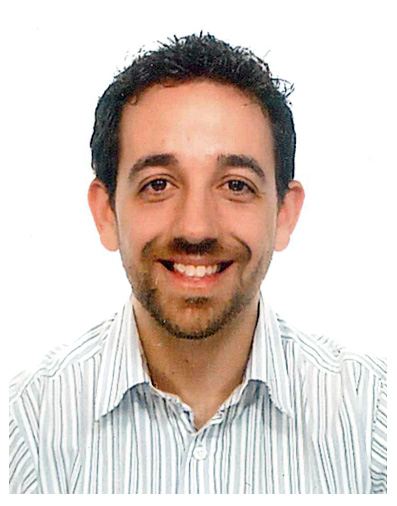
\includegraphics[width=1in,height=1.25in,clip,keepaspectratio]{img/foto_kike}}]
    {Enrique Mart\'i} is a Senior Researcher on Automated Driving at Tecnalia 
    Research and Innovation since 2017. He holds a B.E. degree in Computer
    Sciences (2009), a M.Sc. in Computer Science and Technology (2010) and a 
    PhD (2015) from University Carlos III de Madrid, with a thesis on sensor
    fusion systems sensitive to context information. He stayed as visiting
    researcher in the SUNY University at Buffalo (USA) and in the Centre for
    Maritime Research and Experimentation at La Spezia (Italy), working on 
    coastal surveillance systems based on experimental radar technologies.
    He has more than 10 years of experience in Sensor Fusion and Estimation,
    including participation in national and European R\&D projects and creation
    of commercial information fusion products for large scale surveillance.
    He has worked as Lead Engineer in Navigation and Localization systems in
    a private company building custom UAVs for industrial inspection.
    His research interests include sensor technologies, information fusion,
    estimation techniques, machine learning and optimization applied to
    automated vehicles.
\end{IEEEbiography}

% if you will not have a photo at all:
\begin{IEEEbiography}[{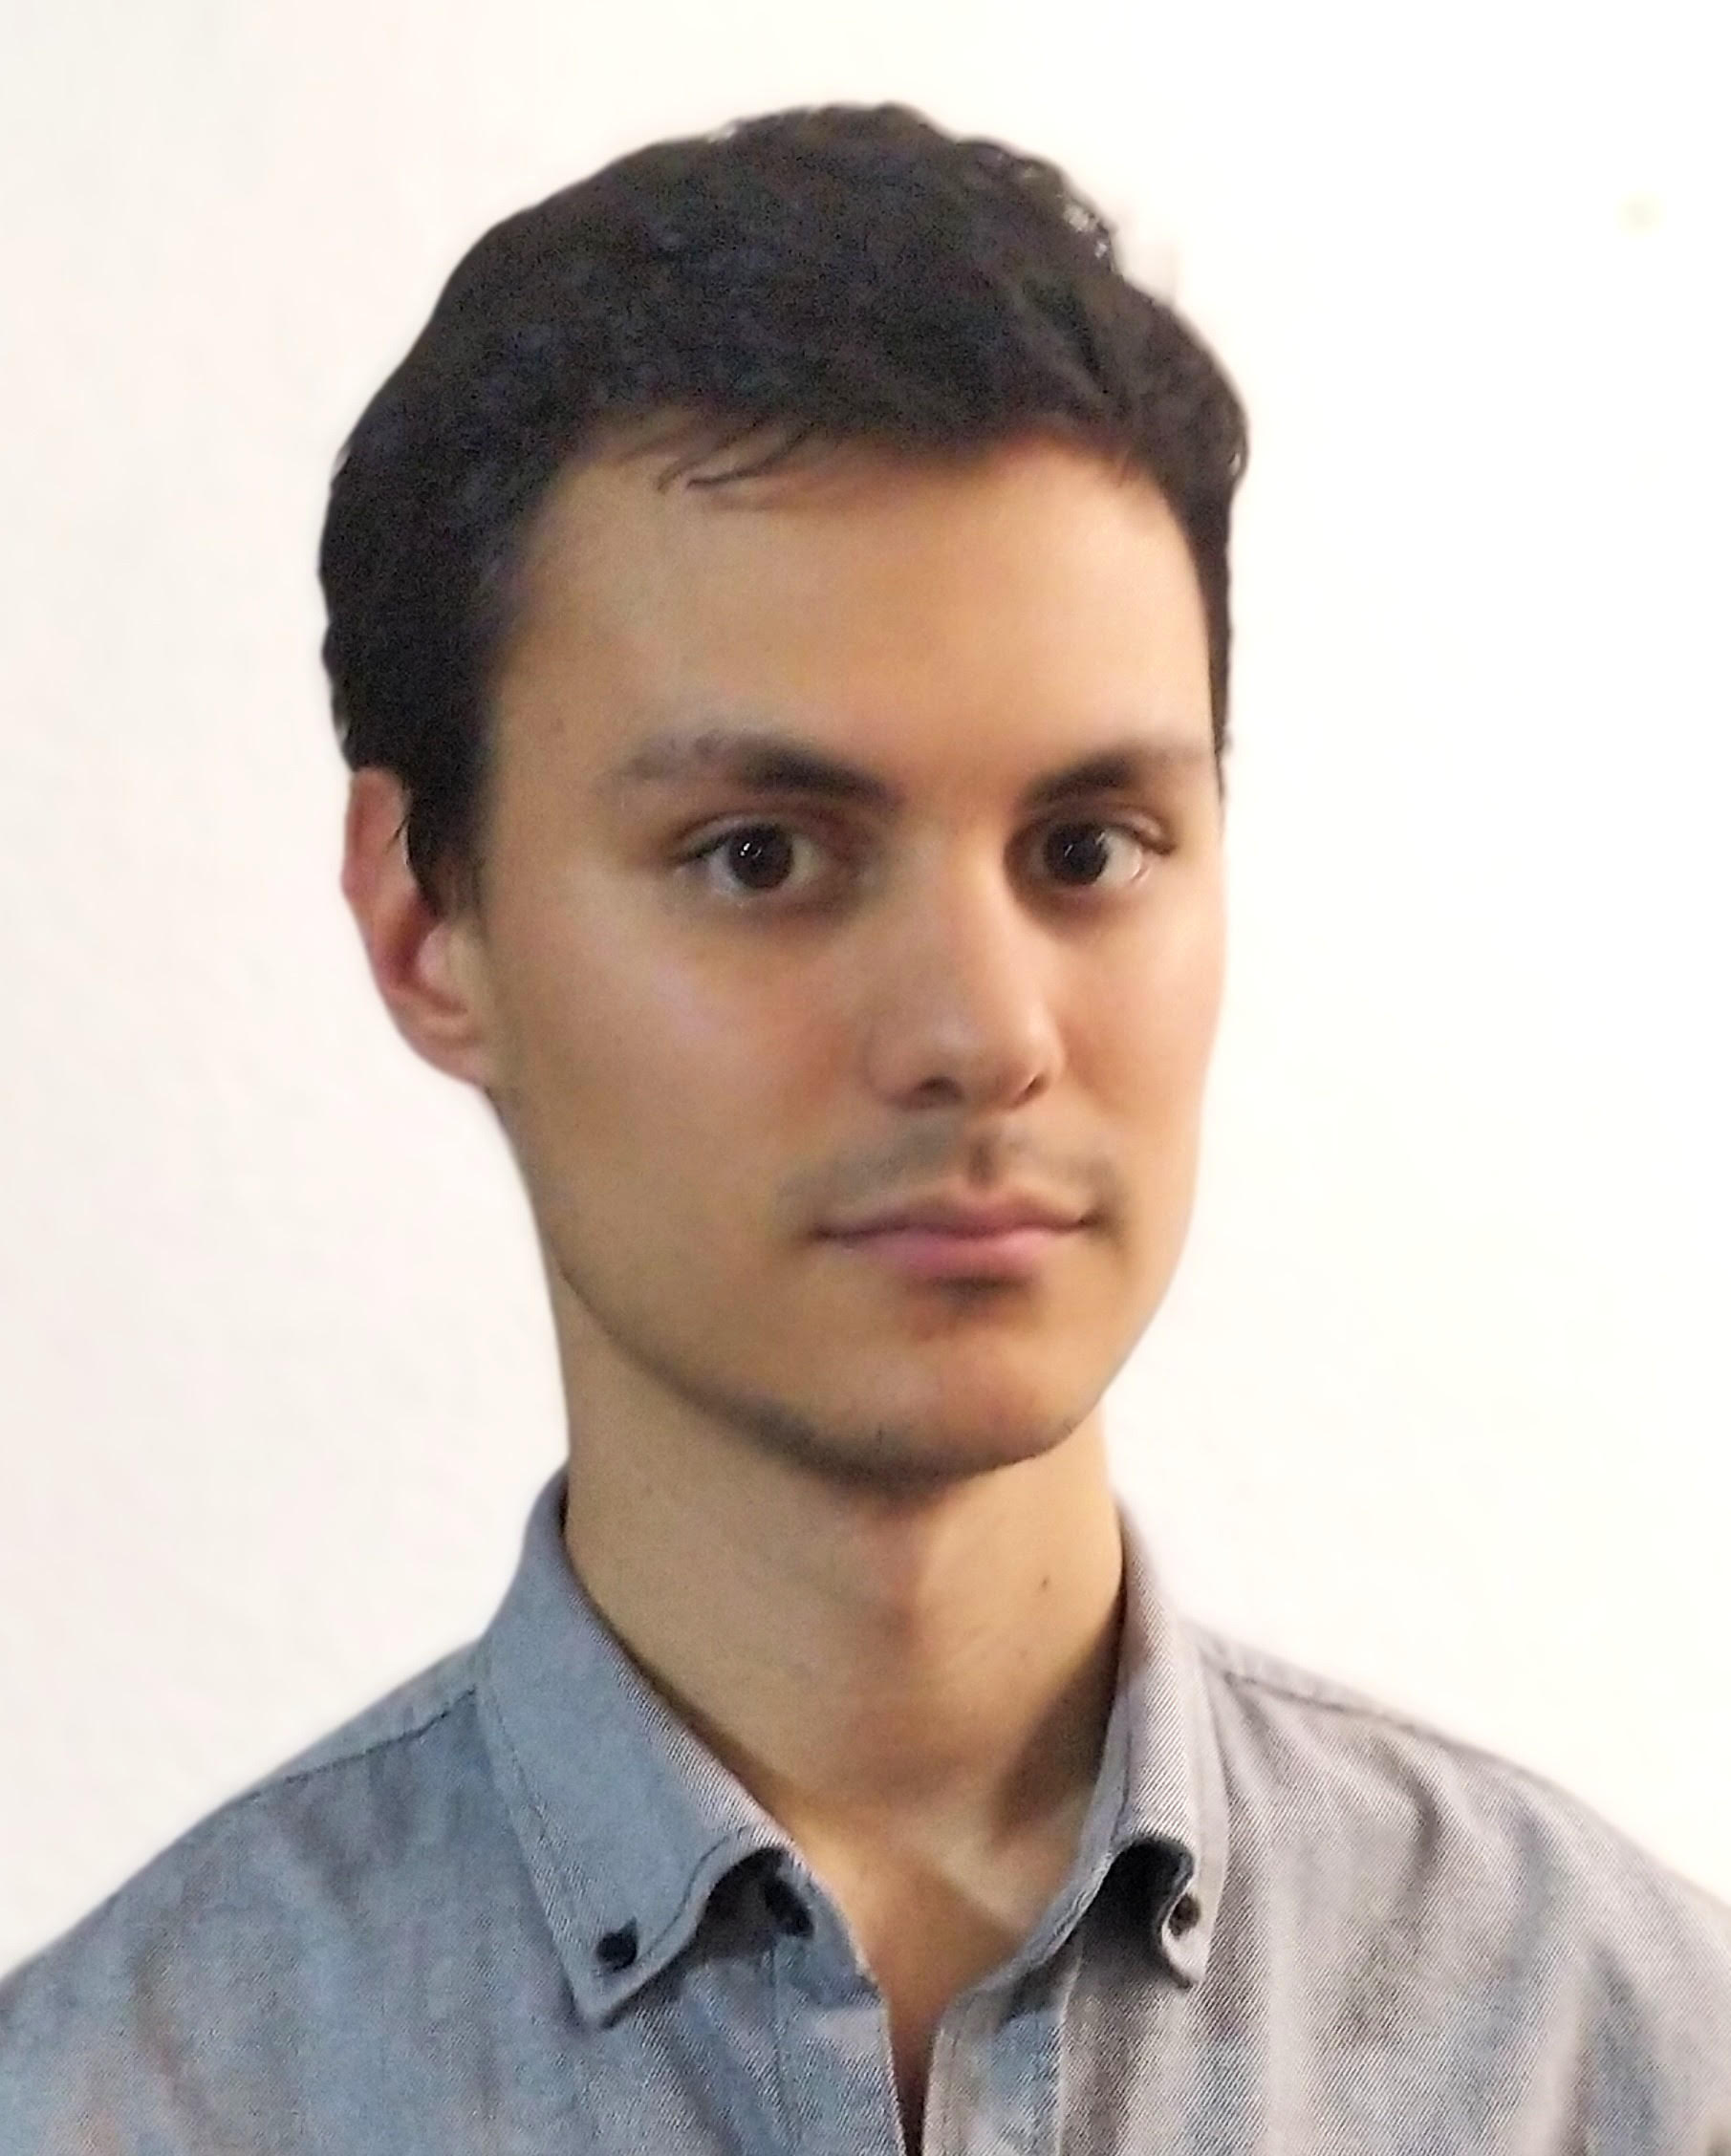
\includegraphics[width=1in,height=1.25in,clip,keepaspectratio]{img/Foto_miguel}}]
{Miguel \'Angel de Miguel}
    was born in Madrid, Spain in 1993. He received the B.S degree in 
    electronics engineering in 2015 and the M.S. degree in industrial
    engineering in 2017, both from University Carlos III de Madrid.
    In 2013 he joined the Intelligent Systems Lab where he has collaborated
    in industrial research projects for three years. Currently, he is a Ph.D. 
    student and an assistant lecturer in the university he studied.
    His research interests include the areas of path planning and control 
    with a focus on applications for autonomous vehicles.
\end{IEEEbiography}


% insert where needed to balance the two columns on the last page with
% biographies
%\newpage
\begin{IEEEbiography}[{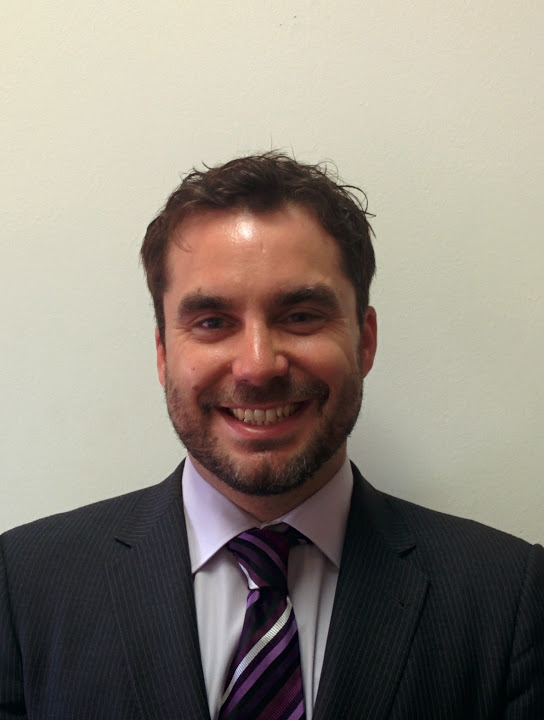
\includegraphics[width=1in,height=1.25in,clip,keepaspectratio]
        {img/foto_fernando}}]
    {Fernando Garc\'ia} is Visiting Professor at Universidad Carlos III de
    Madrid. Where he focuses his researches in Intelligent Vehicles and
    Intelligent 
Transportation Systems involving the use of Computer Vision, Sensor Fusion, and 
Human Factors, as well as Vehicle Communication. He has been recipient of the 
Master in Robotics and Automatics Scholarship at Universidad Carlos III de 
Madrid in 2008, the Barreiros Foundation Award in the domain of Automotive and 
Vehicle Applications in Spain in 2014 and finalist to the best PhD Thesis 
Dissertation Award in the period 2013-2015 given by ITSS Spanish Chapter, and 
the award to the innovation in the automotive sector, diagnosis "Galeria de 
innovación Motortec 2015".  He has organization experience in the ITSS 
conferences  and is member of the BoG and Vice-president of the Spanish Chapter 
of the IEEE-ITSS since January 2017.
He has been involved in more than 40 research projects, 16 of which are funded 
by public entities. He is author of 3 patents and published more than 70 papers 
in international conferences and journals. He spent 10 months as visiting 
researcher in Vislab, at Universidad de Parma, spread in different periods 
(2008, 2011 and 2014). He also stayed as visiting researcher during 4 months at 
SUNY University at Buffalo in 2010. As lecturer, he has given lectures in 
different international Universities such as University of Buffalo, Università 
degli Studi di Parma, Universidad Pontificia Bolivariana de Medellin, 
Universidad de las Fuerzas Armadas de Quito (ESPE), Universidad de La Salle at 
Bogotá, and Universidad Politécnica de Madrid. Moreover, he gives lectures in 
Programming, Computer Vision, Data Fusion, Intelligent Transport Systems and 
Control Engineering.
\end{IEEEbiography}

\begin{IEEEbiography}[{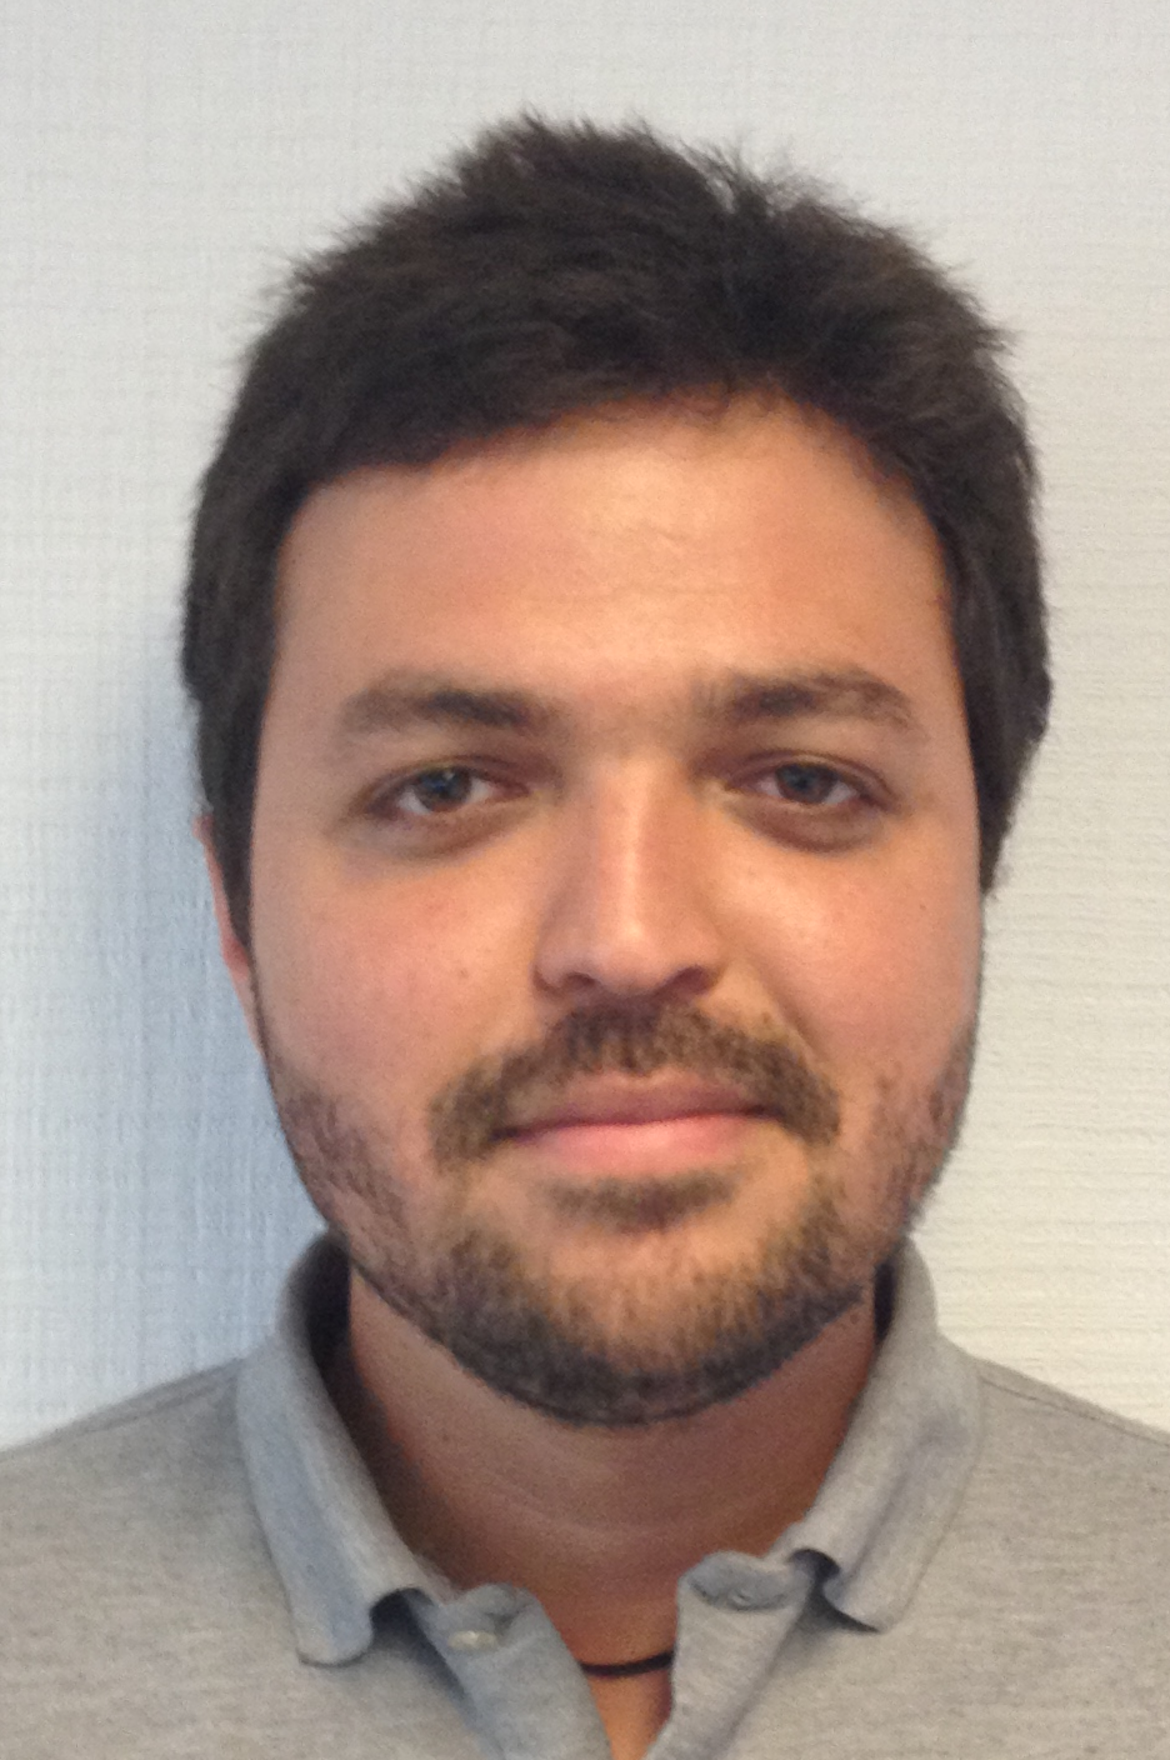
\includegraphics[width=1in,height=1.25in,clip,keepaspectratio]{img/FotoPaperJosh}}]
    {Joshu\'e P\'erez} is a Research leader on Automated Driving at Tecnalia 
    Research and Innovation, since 2015. He received the B.E. degree in 
    electronic engineering from the Sim\'on Bol\'ivar University, Venezuela, in 
    2007. His M.E. degree and his Ph.D. degree from the University Complutense 
    of Madrid were achieved in 2009 and 2012, respectively. He received the 
    best PhD thesis award in intelligent control from the Spanish Committee of 
    Automation (CEA). He has more than 11 years of experience in the 
    Intelligent Transportation System field, where he has been working in 
    national and European projects ranging from ADAS up to fully automated 
    vehicles. His research interests include fuzzy logic, modeling, control, 
    path planning, Cybercars, cooperative maneuvers, automated vehicles, Shared 
    Control, and vehicle standards. He is associate editor of IEEE Intelligent 
    Vehicle Symposium. In 2014, he was guest editors of the IEEE Intelligent 
    Transportation Systems Magazine, in the special issue of ELECTRO-MOBILITY. 
    He has technically led 20+ EU and national projects for demonstrating 
    different ADAS technologies. He has more than 100 publications related to 
    Automated Driving, ADAS and cooperative maneuvers.
\end{IEEEbiography}

% You can push biographies down or up by placing
% a \vfill before or after them. The appropriate
% use of \vfill depends on what kind of text is
% on the last page and whether or not the columns
% are being equalized.

%\vfill

% Can be used to pull up biographies so that the bottom of the last one
% is flush with the other column.
%\enlargethispage{-5in}



% that's all folks
\end{document}


